\documentclass[preprint, 3p, authoryear,review, 12pt]{elsarticle} %review=doublespace preprint=single 5p=2 column
%%% Begin My package additions %%%%%%%%%%%%%%%%%%%

\usepackage[hyphens]{url}

  \journal{Atmospheric Research} % Sets Journal name

\usepackage{lineno} % add
  \linenumbers % turns line numbering on

\usepackage{graphicx}
%%%%%%%%%%%%%%%% end my additions to header

\usepackage[T1]{fontenc}
\usepackage{lmodern}
\usepackage{amssymb,amsmath}
\usepackage{ifxetex,ifluatex}
\usepackage{fixltx2e} % provides \textsubscript
% use upquote if available, for straight quotes in verbatim environments
\IfFileExists{upquote.sty}{\usepackage{upquote}}{}
\ifnum 0\ifxetex 1\fi\ifluatex 1\fi=0 % if pdftex
  \usepackage[utf8]{inputenc}
\else % if luatex or xelatex
  \usepackage{fontspec}
  \ifxetex
    \usepackage{xltxtra,xunicode}
  \fi
  \defaultfontfeatures{Mapping=tex-text,Scale=MatchLowercase}
  \newcommand{\euro}{€}
\fi
% use microtype if available
\IfFileExists{microtype.sty}{\usepackage{microtype}}{}
\usepackage[]{natbib}
\bibliographystyle{plainnat}

\usepackage{graphicx}
\ifxetex
  \usepackage[setpagesize=false, % page size defined by xetex
              unicode=false, % unicode breaks when used with xetex
              xetex]{hyperref}
\else
  \usepackage[unicode=true]{hyperref}
\fi
\hypersetup{breaklinks=true,
            bookmarks=true,
            pdfauthor={},
            pdftitle={Hourly Assimilation of Different Sources of Observations Including Satellite Radiances in a Mesoscale Convective System Case During RELAMPAGO campaign},
            colorlinks=false,
            urlcolor=blue,
            linkcolor=magenta,
            pdfborder={0 0 0}}

\setcounter{secnumdepth}{5}
% Pandoc toggle for numbering sections (defaults to be off)


% tightlist command for lists without linebreak
\providecommand{\tightlist}{%
  \setlength{\itemsep}{0pt}\setlength{\parskip}{0pt}}

% From pandoc table feature
\usepackage{longtable,booktabs,array}
\usepackage{calc} % for calculating minipage widths
% Correct order of tables after \paragraph or \subparagraph
\usepackage{etoolbox}
\makeatletter
\patchcmd\longtable{\par}{\if@noskipsec\mbox{}\fi\par}{}{}
\makeatother
% Allow footnotes in longtable head/foot
\IfFileExists{footnotehyper.sty}{\usepackage{footnotehyper}}{\usepackage{footnote}}
\makesavenoteenv{longtable}


\usepackage[utf8]{inputenc}
\usepackage{booktabs}
\usepackage{longtable}
\usepackage{array}
\usepackage{multirow}
\usepackage{wrapfig}
\usepackage{float}
\usepackage{colortbl}
\usepackage{pdflscape}
\usepackage{tabu}
\usepackage{threeparttable}
\usepackage{threeparttablex}
\usepackage[normalem]{ulem}
\usepackage{makecell}
\usepackage{xcolor}



\begin{document}


\begin{frontmatter}

  \title{Hourly Assimilation of Different Sources of Observations Including Satellite Radiances in a Mesoscale Convective System Case During RELAMPAGO campaign}
    \author[UBA,CIMA,CNRS]{Paola Belén Corrales%
  %
  \fnref{1}}
   \ead{paola.corrales@cima.fcen.uba.ar} 
    \author[UBA,CIMA,CNRS]{V. Galligani}
  
    \author[UBA,CIMA,CNRS]{Juan Ruiz}
  
    \author[INPE]{Luiz Sapucci}
  
    \author[SMN,CONICET]{María Eugenia Dillon}
  
    \author[SMN,CONICET,CNRS]{Yanina García Skabar}
  
    \author[SMN]{Maximiliano Sacco}
  
    \author[NCAR]{Craig S. Schwartz}
  
    \author[Illinois]{Stephen W. Nesbitt}
  
      \affiliation[UBA]{Universidad de Buenos Aires, Facultad de Ciencias Exactas y Naturales, Departamento de Ciencias de la Atmosfera y los Oceanos. Buenos Aires, Argentina.}
    \affiliation[CIMA]{CONICET -- Universidad de Buenos Aires. Centro de Investigaciones del Mar y la Atmosfera (CIMA). Buenos Aires, Argentina.}
    \affiliation[CNRS]{CNRS -- IRD -- CONICET -- UBA. Instituto Franco-Argentino para el Estudio del Clima y sus Impactos (IRL 3351 IFAECI). Buenos Aires, Argentina.}
    \affiliation[SMN]{Servicio Meteorologico Nacional de Argentina.}
    \affiliation[CONICET]{CONICET (Consejo Nacional de Investigaciones Cientificas y Tecnicas).}
    \affiliation[INPE]{National Institute for Space Research, Brazil, Center for Weather Forecasting and Climate Studies.}
    \affiliation[NCAR]{National Center for Atmospheric Research, Boulder, Colorado.}
    \affiliation[Illinois]{Department of Atmospheric Sciences, University of Illinois Urbana--Champaign, Urbana, Illinois.}
    \cortext[cor1]{Corresponding author}
    \fntext[1]{Corresponding Author}
  
  \begin{abstract}
  This paper evaluates the impact of assimilating high-resolution surface networks and satellite observations using the WRF-GSI-LETKF over central and north eastern Argentina where the surface and upper air observing networks are relatively coarse. A case study corresponding to a huge mesoscale convective system (MCS) that developed during November 22, 2018 was used. The accumulated precipitation associated with this MCS was quite high, exceeding 200 mm over northern Argentina and Paraguay. The MCS developed during the Intense Observing Period (IOP) of the Remote sensing of Electrification, Lightning, And Mesoscale/microscale Processes with Adaptive Ground Observations (RELAMPAGO) field campaign. The GSI-4DLETKF data assimilation package is used to produce analyses by assimilating observations every hour with 10-km horizontal grid spacing and a 60-member multiphysics ensemble. Four assimilation experiments are conducted using different sets of observations: CONV, consisting of conventional observations from NCEP's prepBUFR files; AWS, combining CONV and dense automatic surface weather station networks (AWS), SATWND, combining AWS with satellite-derived winds, and RAD, including SATWND; and satellite radiances from different microwave and infrared sensors. The assimilation of observations with high temporal and spatial frequency generates an important impact on the PBL, primarily on the precipitable water content, that leads to the development of deep convection and heavy precipitation closer to the observed in this case study. The assimilation of radiance observations produces a better development of the convection mainly during the mature state of the MCS leading to an increase in the accumulated precipitation. Ensemble forecasts initialized from each experiment were also simulated to evaluate their skill to predict precipitation. The hourly assimilation of the observations in AWS, SATWND, and RAD helped to improve the precipitation forecast.
  \end{abstract}
    \begin{keyword}
    Regional Data Assimilation, Surface Observations, Satellite Observations \sep 
    Regional Data Assimilation, Surface Observations, Satellite Observations
  \end{keyword}
  
 \end{frontmatter}

\hypertarget{introduction}{%
\section{Introduction}\label{introduction}}

Severe weather events cause significant human and economic losses around the world. A large number of these phenomena are associated with the occurrence of deep moist convection, including tornadoes, intense wind gusts, extreme precipitation in short time periods, large hail, and lightning.
Southern South America has one of the highest frequencies in the world of favorable conditions for high-impact meteorological events \citep{brooks2003} and large hail events \citep{cecil2012}, particularly during austral spring and summer.
This is also confirmed by observational evidence and high impact weather reports \citep{matsudo2015, rasmussen2014}. Recently, the Remote sensing of Electrification, Lightning, And Mesoscale/microscale Processes with Adaptive Ground Observations (RELAMPAGO) field campaign \citep{nesbitt2021} has been conducted to investigate the mechanisms for convective initiation and the occurrence of high-impact weather events associated with deep convection in central Argentina.

Forecasting mesoscale meteorological phenomena and particularly deep moist convection is a scientific and technological challenge due to its limited predictability and the difficulties in diagnosing the state of the atmosphere at small spatial and short temporal scales (for example from 1 to 10 kilometers and on the order of minutes). Mesoscale data assimilation (DA) is an approach that can provide appropriate initial conditions for high-resolution numerical forecasts \citep{sun2014} and thus has received increasing attention in the last decades.

For DA methods to be successful, observing networks with sufficient temporal and spatial resolution capable of capturing mesoscale variability should be used \citep{gustafsson2018}. Assimilating information on temperature, moisture, and wind in the planetary boundary layer (PBL) improves mesoscale model initialization, and several authors have reported the resultant beneficial impacts on the PBL structure and the location and timing of precipitating systems (e.g. \citet{wheatley2010}, \citet{ha2014}, \citet{chang2017}, \citet{bae2022}, \citet{banos2021}, \citet{maejima2019}, and \citet{chen2016}).

Particularly relevant for regional mesoscale DA systems in the region of interest is that South America is characterized by a limited number of conventional observations (i.e., radiosondes, surface weather stations) and operational networks that are not dense enough to capture mesoscale details. In this context, analyzing the potential impact of non-conventional sources of observations is essential to improve mesoscale numerical weather prediction (NWP) over South America using DA. There have been only a few published efforts on regional mesoscale DA, but they have all shown promising results \citep[e.g.][]{dillon2016, dillon2021, goncalvesdegoncalves2015}. In particular, \citet{dillon2021} assimilated high resolution surface weather station networks, GOES-16 atmospheric motion vectors (AMVs), and satellite temperature and moisture retrievals over central Argentina with positive impacts. Similar to \citet{gasperoni2018}, \citet{dillon2021} included private weather station networks which are not incorporated in the operational analysis. However, the impact of different observation types on the analysis quality has not been addressed.

The impact of non-conventional high spatial and temporal resolution observations, such as AMVs, has been investigated in the context of regional mesoscale DA. Many studies have focused on the impact of these observations on the prediction of tropical storms (e.g., \citet{wu2014}, \citet{cherubini2006}, and \citet{sawada2019}, and many others). Most of these studies reported an overall positive impact of the assimilation of AMVs for this type of storm. However, some works indicated mixed impacts (e.g. \citet{sawada2019} reported an improvement in the forecast of the track of the storm but a degradation in the forecast intensity). As stated in \citet{zhao2021, zhao2021a}, the impact of assimilating these data on high impact weather events associated with mid-latitude deep convection over land has received relatively less attention. \citet{zhao2021, zhao2021a} assimilated GOES-16 AMVs into a storm-scale three-dimensional variational DA system during three high impact weather events. They reported positive impacts of AMVs on the characterization of the storm environment and improved short range precipitation forecasts. \citet{otsuka2015} and \citet{mallick2020} found a slight improvement in the short-range precipitation forecast due to the storm-scale assimilation of high frequency AMVs.

While the assimilation of radiance observations into global models is well established \citep{eyre2020}, the direct assimilation of radiance data into regional models, however, still remains a challenge due to the sparse data coverage (in the case of polar-orbiting satellite observations), bias correction, and the relatively low model tops used for this application. \citet{bao2015} studied the impact of assimilating cloud-cleared microwave and infrared radiance data polar orbiting instruments on temperature and humidity forecasts over the western USA and found a reduction in the temperature bias at low and mid-levels as a result of the microwave observations but an opposite effect for infrared data. More recently, \citet{zhu2019} studied the impact of assimilating clear sky polar orbiting satellite radiance data within a frequently updated regional system and showed an improvement for all variables, in particular for relative humidity at upper levels. \citet{wang2021} studied the impact of assimilating clear sky radiances in the high-resolution Copernicus European Regional Reanalysis. They reported that satellite radiance observations had a neutral impact on the analyses of geopotential height in the lower troposphere, while a slightly negative impact on the upper troposphere and the stratosphere. They also observed similar results for 3-h forecasts initialized from the analysis but a positive impact on 12 and 24 -h forecasts. Given these mixed results, there is still room to analyze the utility of assimilating radiance observations in a limited-area DA system over land. Moreover, to the best of our knowledge, there are no studies related to the direct assimilation of radiance observations over South America.

The main objective of this work is thus to contribute to the quantification and comparison of the impact of high resolution automatic weather stations, AMVs, and clear-sky satellite radiances, into a mesoscale, frequently-updated ensemble-based regional DA system. This is particularly important in the efforts to improve mesoscale numerical weather prediction (NWP) over South America where the conventional observation network is rather sparse and other sources of information could potentially fill certain gaps. In particular, this paper focuses on the impact in the context of a mid-latitude mesoscale convective system. To reach this goal, several DA experiments are conducted for a case study of a large Mesoscale Convective System (MCS) that developed over Southern South America during Nov 22-23, 2018 during the intense observation period (IOP) of the RELAMPAGO field campaign.

The paper is organized as follows. The DA system, the experimental design, and the observations used are presented in section 2. Results are discussed in section 3 and finally, conclusions are summarized in section 4.

\hypertarget{data-and-methods}{%
\section{Data and Methods}\label{data-and-methods}}

\hypertarget{case-overview}{%
\subsection{Case overview}\label{case-overview}}

Previously to the development of this case study, the center and north of Argentina was immersed in a warm and humid air mass with high values of convective available potential energy (CAPE), as shown by ERA 5 Reanalysis \citep{era5pressure} in Figure \ref{fig:case}a. On Nov 22, 2018 a cold front crossed the center of Argentina (Figure \ref{fig:case}b). This cold front triggered isolated convective cells that rapidly grew upscale into an exceptionally large MCS (Figure \ref{fig:case}d,e). During that day several surface stations reported lightning, strong wind gusts, and heavy rain. To the north of the region, a warm and humid environment contributed to the development of isolated convection that ultimately grew and merged with the MCS (Figure \ref{fig:case}f).
The MCS traveled approximately 2500 km from south to north, dissipating over Paraguay and Southern Brazil after 42 hours.



\begin{figure*}

{\centering 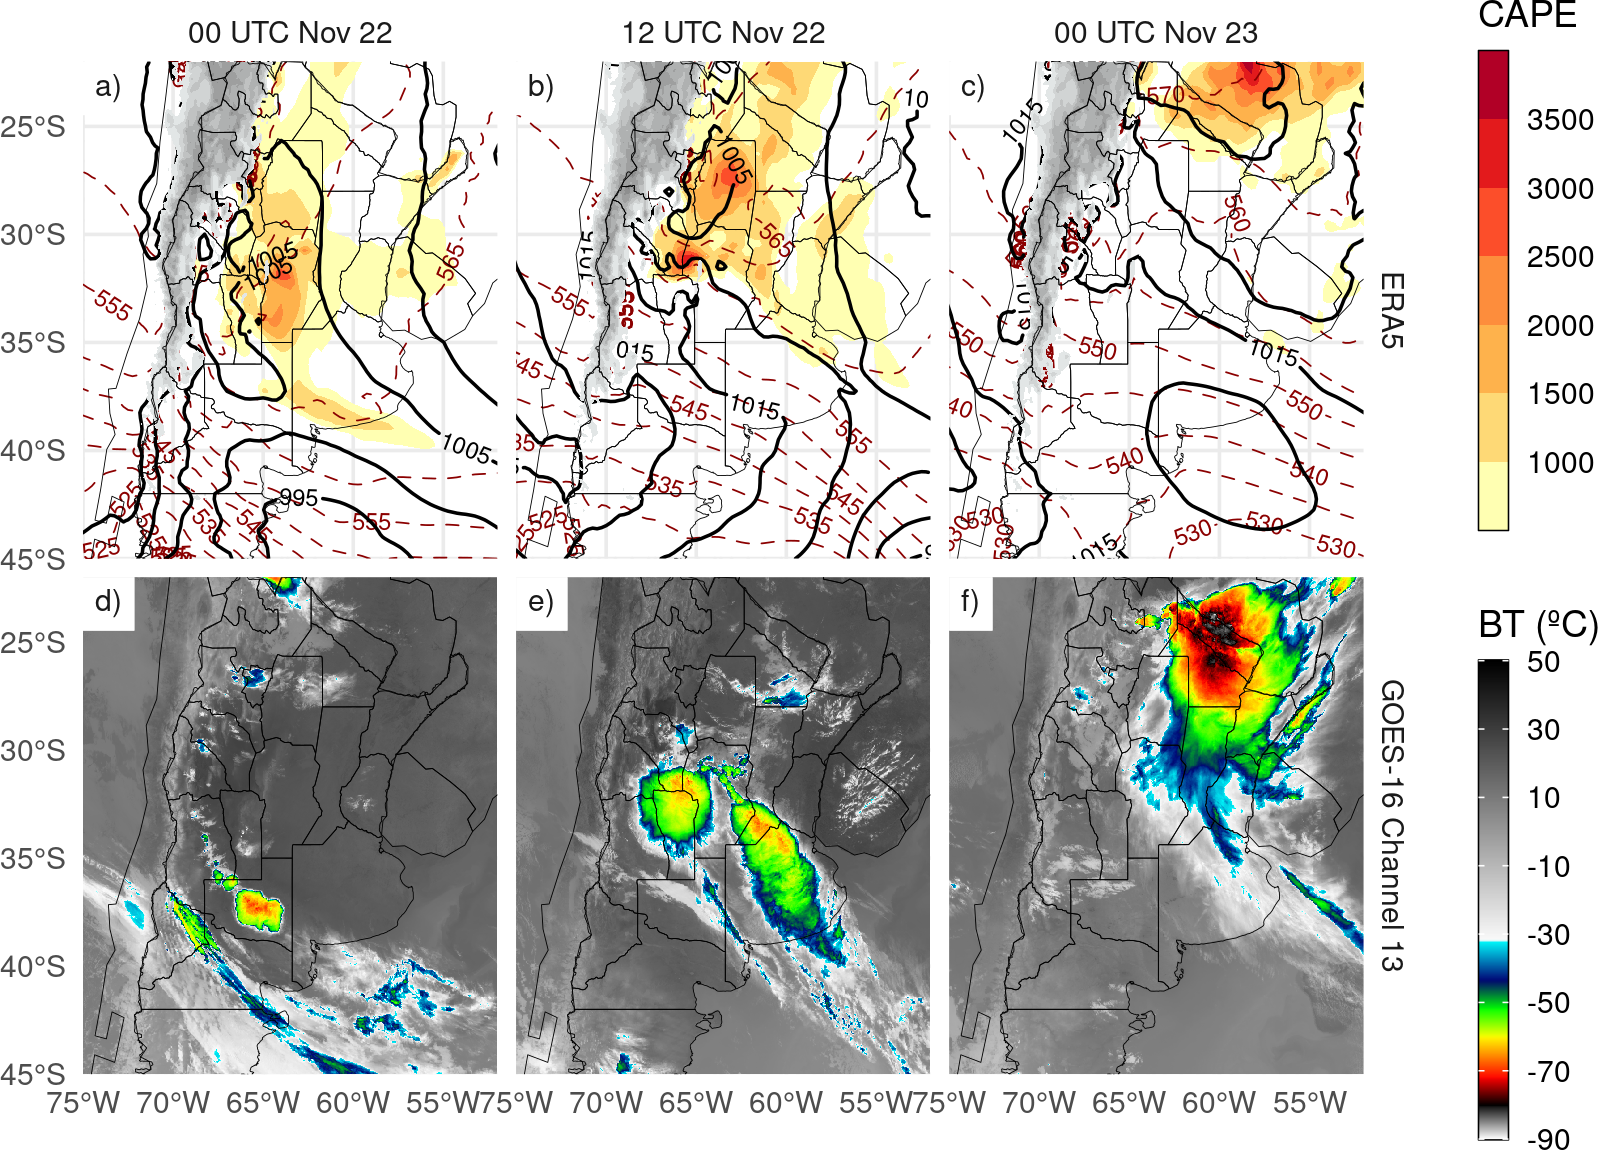
\includegraphics{../figures/case-1} 

}

\caption{ERA5 Reanalysis of sea level pressure (hPa, black contours), 1000-500 hPa thickness (red dashed contours) and convective available potential energy (shaded) and GOES-16 channel 13 brightness temperature for a,d) 00 and b,e) 12 UTC Nov 22 and c,f) 00 UTC Nov 23.}\label{fig:case}
\end{figure*}

\hypertarget{config}{%
\subsection{Data assimilation system configuration}\label{config}}

The forecast model uses the non-hydrostatic Advanced Research version of Weather Research and Forecasting (WRF-ARW V3.9.1, \citet{skamarock2008}).
The horizontal grid spacing is 10 km (150 x 200 grid points) in the horizontal and 37 levels in the vertical with the top of the model at 50 hPa.
The initial and boundary conditions are provided by the Global Forecast System (GFS) analysis (0.25\(^{\circ}\) horizontal grid spacing and 6-hour temporal resolution; \citet{cisl_rda_ds084.1}). In this case, a single nesting approach is used since the resolution gap between the driving model and the regional model is not too large (0.25\(^{\circ}\) or 25 km approximately to 10 km). This approach is also based on recent studies which suggest that using multiple nested domains does not necessarily lead to improved precipitation forecasts in regional domains, particularly in areas of complex terrain (e.g. \citet{liang2019}, \citet{beck2004}). The domain covers the area indicated in Figure \ref{fig:dominio} to capture the development of the MCS during the simulated period.

The analyses are generated using the LETKF implementation (V1.3, \citet{hunt2007}) of the Gridpoint Statistical Interpolation analysis system (GSI V3.8; \citet{shao2016}).
A rapid update cycle approach is implemented with hourly analysis and a centered assimilation window, meaning that all the observations within \(\pm\) 30 minutes of the analysis time are assimilated.
Observations are assimilated in a 4D approach by comparing them with the corresponding first guess state at 10-minute intervals.
For radiance observations, the Community Radiative Transfer Model version 2.3 (CRTM; \citet{han2006}) is used as an observation operator to calculate model-simulated brightness temperatures.

A 60-member ensemble is used where the initial ensemble mean and the mean boundary conditions are taken from the GFS deterministic analysis. A set of 60 perturbations are randomly generated to perturb the initial state as well as the boundary conditions during the length of the experiment. Perturbing the boundary conditions helps to reduce the impact of errors in the driving global model and helps to keep a larger ensemble spread throughout the domain and during the length of the experiment \citep{ouaraini2015}. The perturbations are generated as scaled differences between two random atmospheric states obtained from the Climate Forecast System Reanalysis (CFSR) data with 0.5\(^{\circ}\) horizontal grid spacing with a smooth time evolution as in \citet{necker2020} and \citet{maldonado2021}. In this way, the nearly hydrostatic and geostrophic equilibrium of larger scales is preserved. The random perturbations used are the same across experiments to ensure that the differences between experiments are only related to changes in the number and type of assimilated observations.

A multi-physics scheme is used to better represent the uncertainty in the model formulation within the DA system. 9 different model configurations are generated consisting of the combination of 3 moist convection schemes (Kain--Fritsch \citep{kain2004}, Grell--Freitas \citep{grell2013}, and Betts--Miller--Janjic \citep{janjic1994}) and 3 planetary boundary layer schemes (Yonsei University Scheme \citep{hong2006}, Mellor--Yamada--Janjic Scheme \citep{janjic1994}, and Mellor--Yamada Nakanishi Niino \citep{nakanishi2009}). The distribution of these schemes among the 60 ensemble members is outlined in Table \ref{tab:miembros-desc}. The multi-physics approach is also introduced in order to represent the uncertainty associated with the more relevant physical processes that are not resolved by the model. All ensemble members use the same land-surface model (Noah-MP, \citet{chen2001}), microphysics (WRF single-moment 6--class scheme \citep{hong2006a}), and radiation processes (RRTMG shortwave and longwave scheme \citep{iacono2008}) parameterizations.

\begin{table}

\caption{\label{tab:miembros-desc}Generation of the 60-member multi-physics ensemble as a combination of Cumulus and PBL parameterizations.}
\centering
\fontsize{6}{8}\selectfont
\begin{tabular}[t]{c>{\centering\arraybackslash}p{7em}>{\centering\arraybackslash}p{7em}>{\centering\arraybackslash}p{7em}}
\toprule
\multicolumn{1}{c}{ } & \multicolumn{3}{c}{PBL} \\
\cmidrule(l{3pt}r{3pt}){2-4}
Cumulus & MYJ & MYNN2 & YSU\\
\midrule
BMJ & 5, 14, 23, 32, 41, 50, 59 & 8, 17, 26, 35, 44, 53 & 2, 11, 20, 29, 38, 47, 56\\
GF & 6, 15, 24, 33, 42, 51, 60 & 9, 18, 27, 36, 45, 54 & 3, 12, 21, 30, 39, 48, 57\\
KF & 4, 13, 22, 31, 40, 49, 58 & 7, 16, 25, 34, 43, 52 & 1, 10, 19, 28, 37, 46, 55\\
\bottomrule
\end{tabular}
\end{table}

To reduce the effect of spurious correlations in the estimation of error covariances, a horizontal localization radius of 180 km and a vertical localization radius of 0.4 (in log pressure coordinates) is used as in \citet{dillon2021} for all types of observations.
A relaxation-to-prior spread inflation \citep{whitaker2012} is applied with an inflation parameter \(\alpha=0.9\) following \citet{maldonado2020} to mitigate the impact of sampling errors and to consider model errors not accounted for by the multi-model ensemble approach.



\begin{figure}
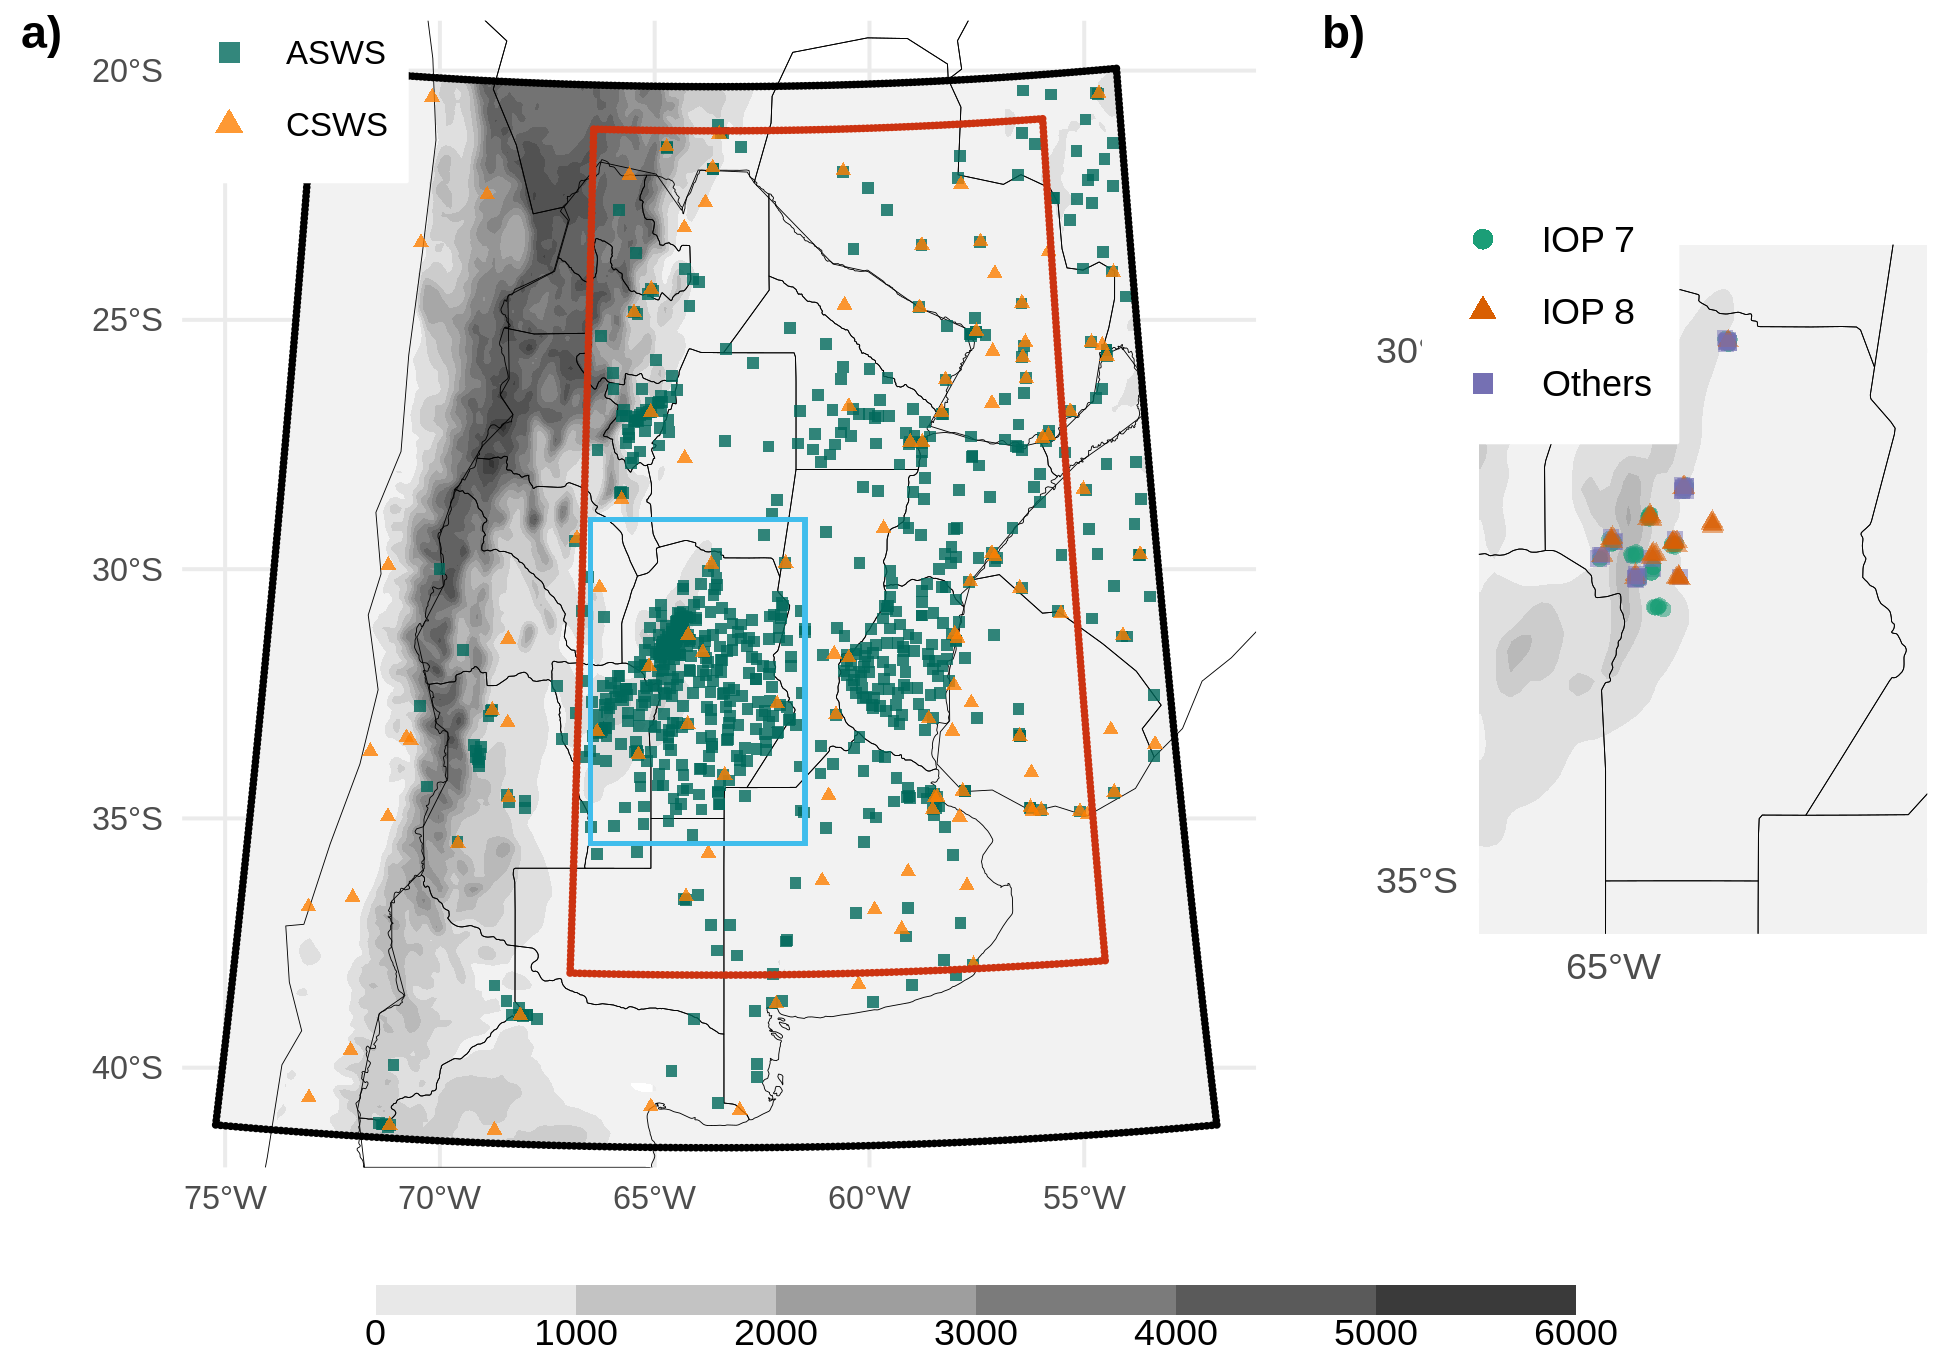
\includegraphics[width=0.98\linewidth]{../figures/dominio-1} \caption{a) The domain used for the simulations (black box), the inner domain used for the experiment comparison (red box), the region shown in b) (light blue box), and the locations of Automatic Weather Stations (AWS, green squares) and Conventional Surface Weather Stations (CSWS, orange triangles). b) Locations of radiosonde launches during RELAMPAGO. Green dots correspond to radiosondes launched during IOP 7, orange triangles are radiosondes launched during IOP 8, and purple squares are radiosondes launched outside the IOP missions. The topography in meters is also shown (shaded).}\label{fig:dominio}
\end{figure}

\hypertarget{observations}{%
\subsection{Observations}\label{observations}}

\hypertarget{conventional}{%
\subsubsection{Conventional}\label{conventional}}

The conventional observations used are part of the Global Data Assimilation System (GDAS) data stream. Conventional observations included in the Binary Universal Form for Representation of Meteorological Data (PREPBUFR) files generated at the National Centers for Environmental Prediction (NCEP) are assimilated. These consist of surface observations from 117 Conventional Surface Weather Stations (CSWS), ships, and upper-air observations from 13 radiosondes sites and aircraft. The orange triangles in Figure \ref{fig:dominio}a indicate the location of the surface stations included in this experiment. The frequency of these observations varied between 1 hour for surface stations and 12/24 hours for radiosondes. Wind surface observations over oceans (ASCATW) come from scatterometers and are also included in the PREPBUFR files.

Table \ref{tab:table-obs} lists all the observation types (i.e., surface pressure, temperature, specific humidity, and wind) available for each source, together with their associated errors. The observation errors were specified following the GSI default configuration. In some cases, the error varies with height and depends on the specific platform (aircraft and satellite-derived wind). In terms of quality control, a gross check was performed by the observation operator by comparing the innovation (the difference between the observation and the model-simulated observation based on the first-guess) with a predefined threshold that depends on the observation error (also included in Table \ref{tab:table-obs}).

\hypertarget{aws-networks}{%
\subsubsection{AWS networks}\label{aws-networks}}

Data from 866 Automatic Weather Stations (AWS) that are part of 17 public and private surface networks over Southern South America are also assimilated. The dataset used in this study has been obtained from the RELAMPAGO Data Set repository \citep{garcia2019}. These stations are indicated as green squares in Figure \ref{fig:dominio}a. They have higher spatial coverage than the CSWS and a sampling frequency of 10 minutes in most cases. All stations measure temperature, but only 395 stations provide humidity, 422 provide pressure, and 605 provide wind information.
Observation errors used to assimilate these observations are the same as for the CSWS (see Table \ref{tab:table-obs}).

\hypertarget{satellite-derived-winds}{%
\subsubsection{Satellite-derived winds}\label{satellite-derived-winds}}

Satellite-derived wind observations are also included in the PREPBUFR files available every 6 h, and consist of estimations from GOES-16 (using the visible, infrared, and water vapor channels) and METEOSAT 8 and 11 (using the visible and water vapor channels). Due to the domain covered by each of these satellites, GOES-16 is the primary source of satellite-derived winds (99 \% of the observations). Observation errors used to assimilate these observations follow the GSI default configuration and are indicated in Table \ref{tab:table-obs}.

\begin{table}

\caption{\label{tab:table-obs}Characteristics of the assimilated observations: The code for each observation type and its source, the available variables, the observation error, and the gross check thresholds used.}
\centering
\fontsize{6}{8}\selectfont
\begin{tabular}[t]{>{\raggedright\arraybackslash}p{3.5em}>{\raggedright\arraybackslash}p{4.5em}>{\raggedright\arraybackslash}p{5em}>{\raggedright\arraybackslash}p{7em}>{\raggedright\arraybackslash}p{7em}}
\toprule
Code & Platform & Variable & Error & Gross check\\
\midrule
 &  & Pressure & 1-1.6 $hPa^*$ & 3.6 $hPa$\\

 &  & Temperature & 1.5 $K$ & 7 $K$\\

 &  & Specific humidity & 20 \% & 8 $gKg^{-1}$\\

\multirow{-4}{3.5em}{\raggedright\arraybackslash CSWS   AWS} & \multirow{-4}{4.5em}{\raggedright\arraybackslash Surface weather stations} & Wind & 2.2 $ms^{-1}$ & 6 $ms^{-1}$\\
\cmidrule{1-5}
 &  & Pressure & 1.1-1.2 $hPa^{**}$ & 4 $hPa$\\

 &  & Temperature & 0.8-1.5 $K^*$ & 8 $K$\\

 &  & Specific humidity & 20 \% & 8 $gKg^{-1}$\\

\multirow{-4}{3.5em}{\raggedright\arraybackslash ADPUPA} & \multirow{-4}{4.5em}{\raggedright\arraybackslash Radiosondes} & Wind & 1.4-3 $ms^{-1}$* & 8 $ms^{-1}$\\
\cmidrule{1-5}
 &  & Temperature & 1.47-2.5 $K^+$ & 7 $K$\\

\multirow{-2}{3.5em}{\raggedright\arraybackslash AIRCFT} & \multirow{-2}{4.5em}{\raggedright\arraybackslash Aircrafts} & Wind & 2.4-3.6 $ms^{-1+}$ & 6.5-7.5 $ms^{-1+}$\\
\cmidrule{1-5}
ASCATW & Advanced Scatterometers & Wind & 1.5 $ms^{-1}$ & 5 $ms^{-1}$\\
\cmidrule{1-5}
 &  & Pressure & 1.3 $hPa$ & 4 $hPa$\\

 &  & Temperature & 2.5 $K$ & 7 $K$\\

 &  & Specific humidity & 20 \% & 8 $gKg^{-1}$\\

\multirow{-4}{3.5em}{\raggedright\arraybackslash SFCSHP} & \multirow{-4}{4.5em}{\raggedright\arraybackslash Ships and Buoys} & Wind & 2.5 $ms^{-1}$ & 5 $ms^{-1}$\\
\cmidrule{1-5}
SATWND & Satellite-derived winds & Wind & 3.8-8 $ms^{-1*+}$ & 1.3-2.5 $ms^{-1+}$\\
\bottomrule
\multicolumn{5}{l}{\rule{0pt}{1em}\textsuperscript{*} Observation error varied with height.}\\
\multicolumn{5}{l}{\rule{0pt}{1em}\textsuperscript{**} Observations above 600 hPa are rejected.}\\
\multicolumn{5}{l}{\rule{0pt}{1em}\textsuperscript{+} Observation error depends on the report type.}\\
\end{tabular}
\end{table}

\hypertarget{sat}{%
\subsubsection{Satellite radiances}\label{sat}}

Satellite radiances available through the GDAS data stream, consisting of infrared and microwave observations, are used in this study. This includes the Advanced Microwave Sounding Unit - A (AMSU-A), Microwave Humidity Sounder (MHS), and 2 multispectral sensors; the Atmospheric Infrared Sounder (AIRS) and the Infrared Atmospheric Sounding Interferometer (IASI) over several satellite platforms (see Table \ref{tab:table-rad}). Since the regional domain is located in the mid-latitudes and the satellite platforms of interest are on polar orbits, each sensor scans the area only twice a day with a spatial coverage depending on the satellite swath. For this reason, the number of satellite observations varied significantly among cycles. In particular, the multispectral sensors provided between 100 and 1000 observations for every scan every 12 hours, contributing 88 \% of the total amount of assimilated radiances in our experiment. The vertical location of each radiance observation was estimated as the model level at which its weighting function was maximized as calculated by CRTM. The multispectral sensors have good vertical coverage and are able to sense from the lower troposphere up to the lower stratosphere.

The channels adopted for assimilation and their associated errors were defined taking into account the low model top (50 hPa). The data preprocessing, which is an essential step in the assimilation of radiances, was performed within the GSI system for each sensor specifically. First, a spatial data thinning is applied using a 60 km grid following \citet{singh2016}, \citet{jones2013}, and \citet{lin2017a}, where the observations to be assimilated are chosen based on their distance to the model grid points, the observation quality (based on available data quality information), and the number of available channels (from the same pixel and sensor) that passed the quality control. Also, observations over the sea are preferred to those over land or snow \citep{hu2018}.

The thinned observations were then bias corrected. The bias correction (BC) has an air-mass dependent and an angle-dependent component \citep{zhu2014} and it is calculated as a multi-linear function of N predictors \(p_i(x)\), with associated coefficients \(\beta_i\). Then, the bias corrected brightness temperature (\(BT_{bc}\)) can be obtained as:

\begin{equation}
  \mathrm{\mathit{BT_{bc}} =\mathit{ BT} + \sum_{i = 0}^{N} \beta_i p_i (x)}
  \label{eq:eq1}
\end{equation}

GSI has a constant offset bias correction term (\(p_0 = 1\)) and the remaining predictors are the cloud liquid water content (CLW), the temperature lapse rate at the pressure of maximum weight, the square of the temperature lapse rate at the pressure of maximum weight, and the emissivity sensitivity. Scan angle-dependent bias is modeled as a 4th-order polynomial \citep{zhu2014}.

In the GSI system, the \(\beta_i\) coefficients are trained using a variational estimation method which solves the \(\beta_i\) that provides the best fit between the simulation and the observations. The coefficients were initialized at 18 UTC Nov 18, 2018 with the GFS system coefficients. The assimilation system was configured to use a constant background error variance of 0.01 to avoid large adjustments in the estimated coefficients at each time.

In our experiments, only clear-sky observations are used. For microwave radiances, observations potentially contaminated by clouds are detected using the scattering and Liquid Water Path (LWP) indexes \citep{weston2019, zhu2016}. For the infrared channels, cloud contaminated observations are detected using the transmittance profile calculated within the CRTM algorithms. Moreover, GSI checks the difference between the observations and simulated brightness temperature with height to detect cloudy pixels. Additionally, the GSI quality control for infrared sensors looks for observations over water with a large zenith angle (over 60°) to reject channels near the visible range that can be contaminated with reflection. It also performs an emissivity check for observations over land for both infrared and microwave radiances.

\begin{table}

\caption{\label{tab:table-rad}List of the available sensors over several platforms, the number of accepted channels for the assimilation, and the percentage of assimilated observations calculated over all radiance observations and all cycles.}
\centering
\fontsize{7}{9}\selectfont
\begin{tabu} to \linewidth {>{\raggedright}X>{\raggedright}X>{\raggedleft}X>{\raggedright}X}
\toprule
Sensor & Platform & Assimilated channels & Percentage over total\\
\midrule
AIRS & AQUA & 52 & 31.63 \%\\
\cmidrule{1-4}
 & NOAA15 & 2 & 3.31 \%\\
\cmidrule{2-4}
 & NOAA18 & 2 & 4.45 \%\\
\cmidrule{2-4}
\multirow[t]{-3}{*}{\raggedright\arraybackslash AMSUA} & METOP-A & 2 & 2.08 \%\\
\cmidrule{1-4}
 & METOP-A & 66 & 52.72 \%\\
\cmidrule{2-4}
\multirow[t]{-2}{*}{\raggedright\arraybackslash IASI} & METOP-B & 68 & 3.47 \%\\
\cmidrule{1-4}
 & NOAA19 & 2 & 0.68 \%\\
\cmidrule{2-4}
 & METOP-A & 3 & 0.8 \%\\
\cmidrule{2-4}
\multirow[t]{-3}{*}{\raggedright\arraybackslash MHS} & METOP-B & 3 & 0.85 \%\\
\bottomrule
\end{tabu}
\end{table}



\begin{figure}
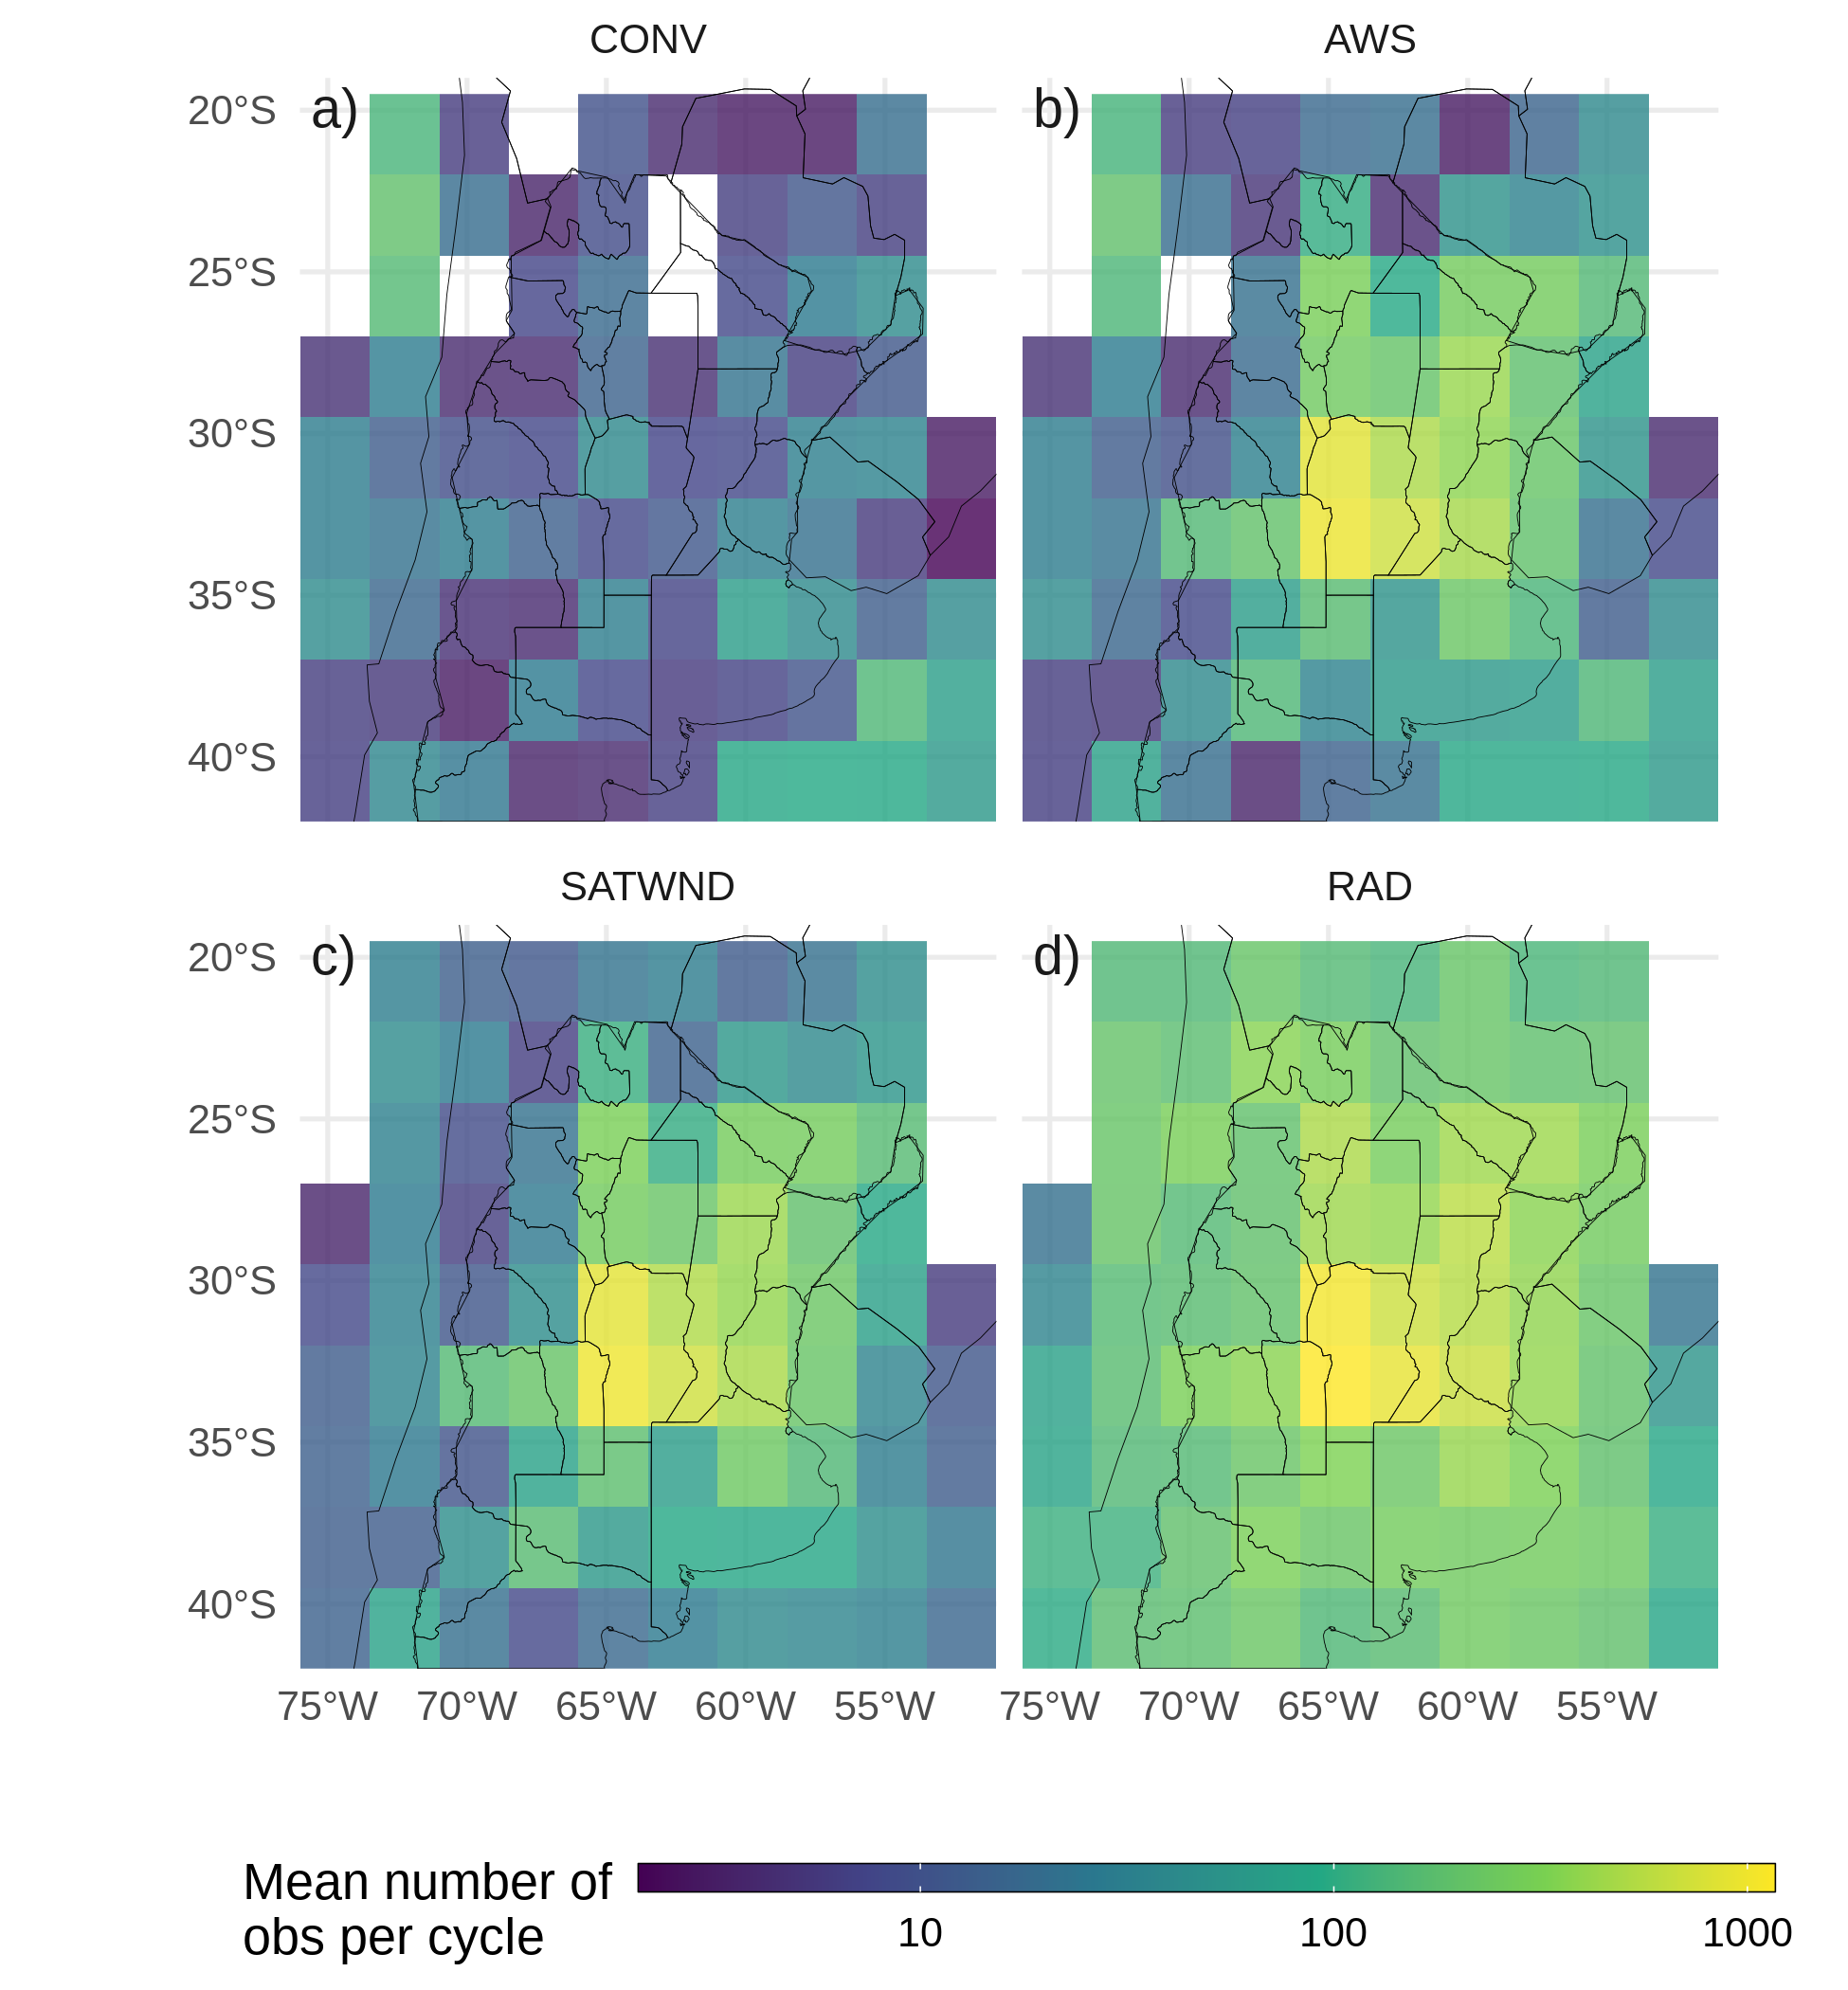
\includegraphics[width=1\linewidth]{../figures/obs-horizontal-1} \caption{Horizontal spatial distribution of the mean available observations per analysis cycle for the a) CONV, b) AWS, c) SATWND, and d) RAD experiments calculated over 2.5\(^{\circ}\) boxes.}\label{fig:obs-horizontal}
\end{figure}



\begin{figure*}
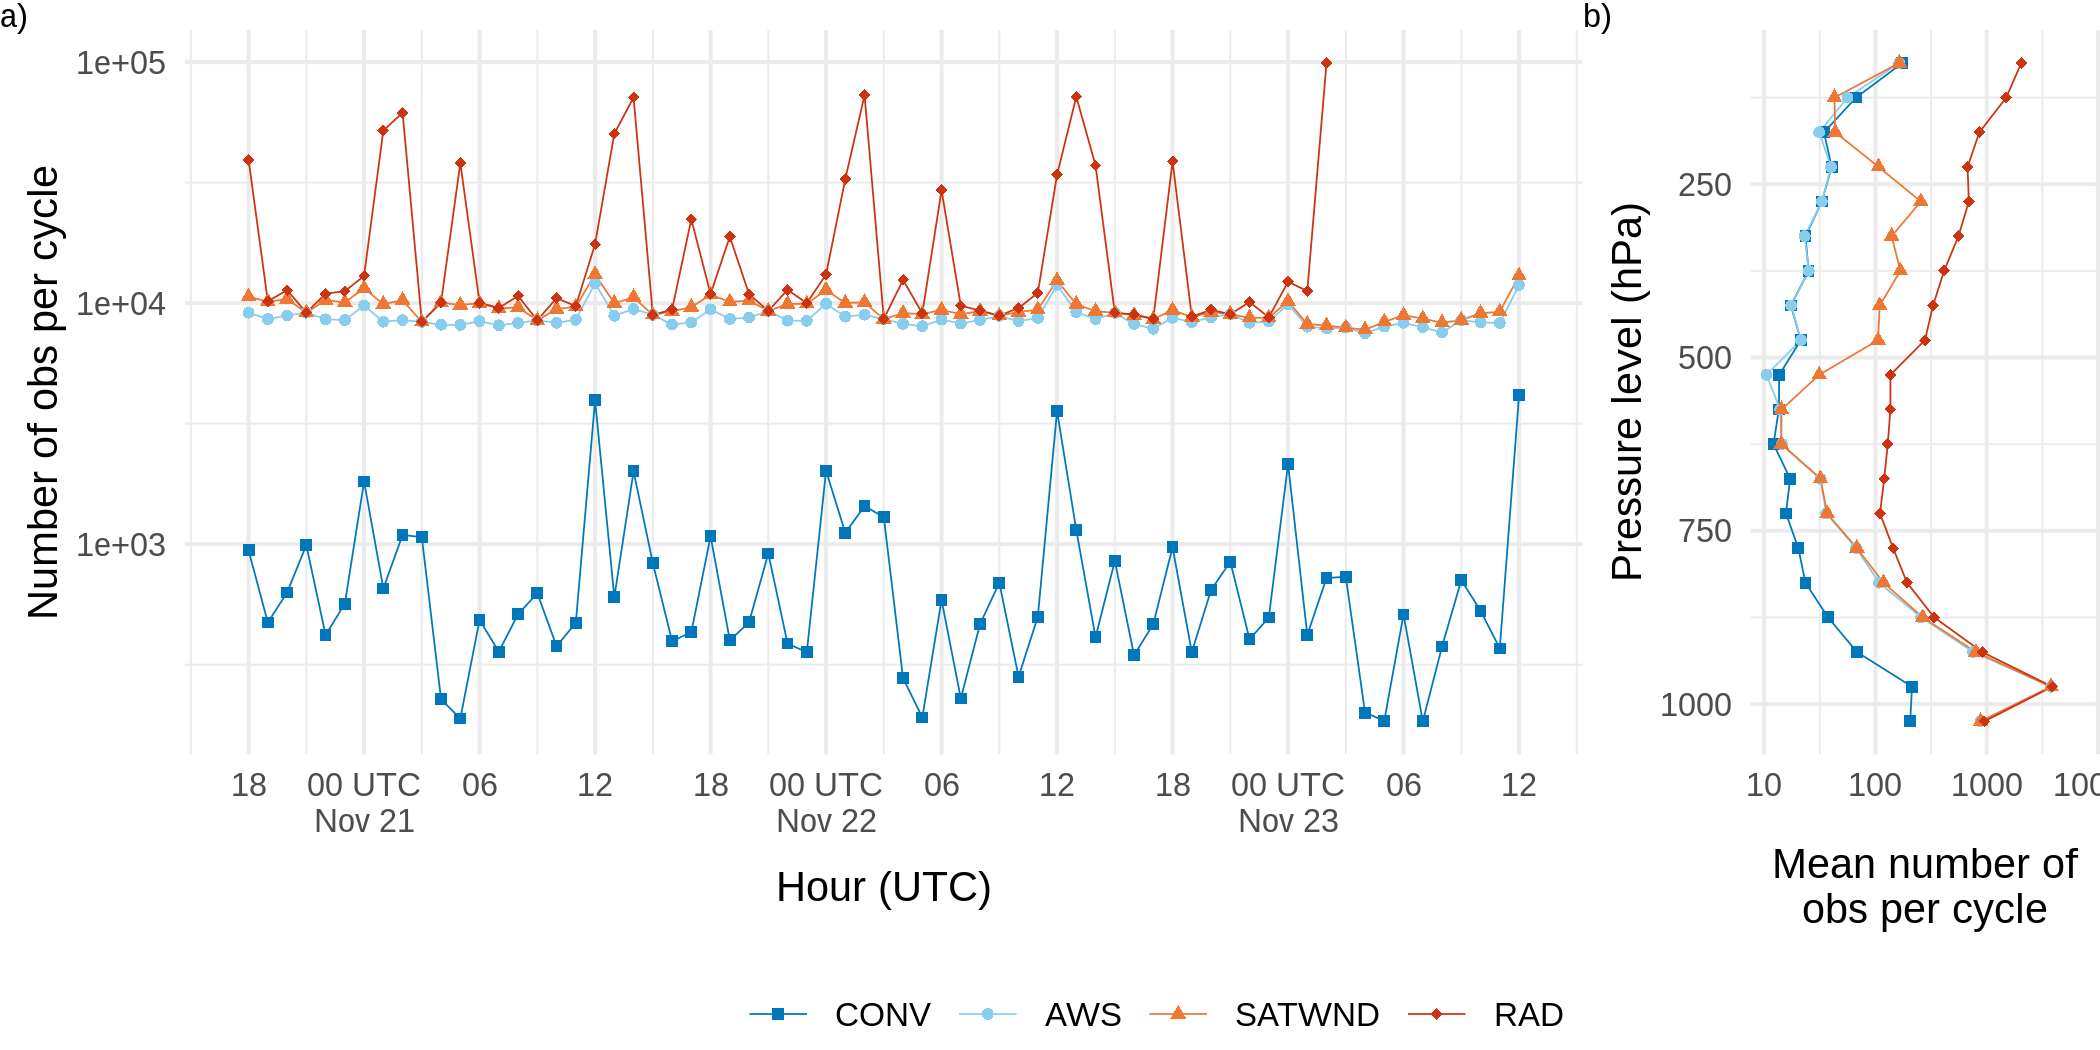
\includegraphics{../figures/obs-cycle-1} \caption{a) Number of assimilated observations per cycle and b) time averaged number of assimilated observations per cycle divided into 50 hPa-depth vertical layers for the CONV (blue squares and line), AWS (light blue dots and line), SATWND (orange triangles and line) and RAD (red diamonds and line) experiments.}\label{fig:obs-cycle}
\end{figure*}

\hypertarget{validation-dataset}{%
\subsubsection{Validation dataset}\label{validation-dataset}}

To evaluate the performance of the ensemble-based DA system presented in this article, the following observational datasets were used:

\begin{itemize}
\item
  ERA5 hourly data on pressure levels from 1959 to present \citep{era5pressure}. The variables of interest (air temperature, humidity and wind) were interpolated to the model grid to compare them with the analysis of each experiment.
\item
  The Multi-Network Composite Highest Resolution Radiosonde Data \citep{sondeos} from the RELAMPAGO field campaign database consisting of high-resolution radiosondes launched from several locations during the IOPs along with the operational radiosondes. Only the soundings that did not enter the assimilation system were used for validation. The experiment period covers IOP missions 7 and 8, during which 74 radiosondes were launched in a small area near the center of the experimental domain (Figure \ref{fig:dominio}b).
\item
  The Satellite precipitation estimation IMERG Final Run with 0.01\(^{\circ}\) spatial resolution and 30 minutes temporal resolution \citep{huffman2018} was used as a reference state to validate the skill of 1-hour forecasts to represent the precipitation over the domain.
\item
  Radar observations are used to perform a qualitative and visual assessment of the convective features. The data comes from 9 radars located in the domain and is provided by the Argentine C-band Doppler dual-polarization weather radar network \citep{deelia2017} with a temporal frequency of 10 minutes. For this work, only the maximum reflectivity in the column (COLMAX) closest to the analysis time was used.
\end{itemize}

\hypertarget{exp}{%
\subsection{Experimental design}\label{exp}}

To investigate the impact of different observations upon the analysis, four DA experiments were performed using different observation sets (Table \ref{tab:table-exp}). The CONV experiment uses only conventional observations from PREPBUFR. In a second experiment, referred to as AWS, all the observations included in CONV are assimilated plus the 10-minute frequency surface observations from AWS. In the third experiment, referred to as SATWND, the observations from the AWS experiment along with the satellite-derived winds are assimilated. Finally, a fourth experiment referred to as RAD assimilates all available clear-sky radiances from sensors onboard polar orbiting satellites as described in section \ref{sat}.

\begin{table}

\caption{\label{tab:table-exp}Observation types assimilated in each experiment.}
\centering
\begin{tabu} to \linewidth {>{\raggedright\arraybackslash}p{8em}>{\centering\arraybackslash}m{2.5em}>{\centering\arraybackslash}m{2.5em}>{\centering\arraybackslash}m{3em}>{\centering\arraybackslash}m{3em}}
\toprule
Obs type & CONV & AWS & SATWND & RAD\\
\midrule
Conventional (PREPBUFR) & x & x & x & x\\
Conventional (AWS) &  & x & x & x\\
Satellite-derived winds &  &  & x & x\\
Radiances &  &  &  & x\\
\bottomrule
\end{tabu}
\end{table}

The horizontal distribution of the average number of assimilated observations per cycle in each experiment is shown in Figure \ref{fig:obs-horizontal}. The larger number of assimilated observations over the center and east of the domain corresponds to the AWS observations. In Figure \ref{fig:obs-cycle}a the number of assimilated observations over time is shown. Local maxima at 12 and 00 UTC found mainly in CONV are attributed to operational soundings. The strong variability in the number of radiance observations per cycle is also noticeable and depends on the satellite coverage. The maxima at 13-14 and 01-02 UTC in RAD correspond to the contribution of the multispectral sensors. The vertical distribution of the mean number of observations per cycle (Figure \ref{fig:obs-cycle}b) shows a maximum in low levels due to the AWS observations. Satellite-derived winds are maximized at the upper troposphere (between 500-250 hPa). Above 850 hPa, most of the observations correspond to radiance observations.

All the assimilation experiments start at 18 UTC Nov 20, 2018 and continue until 12 UTC Nov, 23 (totaling 67 hours/assimilation cycles). The initial 60-member ensemble is generated as explained in section \ref{config} from a spin-up run without assimilating observations performed between 12 UTC and 18 UTC Nov, 20 (Figure \ref{fig:cycle}).

Ensemble forecasts initialized from the different analysis experiments at 00 and 06 UTC Nov 22 were performed to evaluate the impact of the different observing networks on short range precipitation forecasts. Both forecasts are integrated until 12 UTC Nov 23. All forecasts use the same domain and ensemble configuration as the analysis. The boundary conditions for the ensemble members are generated by adding random perturbations to the GFS deterministic forecast (0.25\(^{\circ}\) horizontal grid spacing and 6-hour temporal resolution; \citet{cisl_rda_ds084.1}).



\begin{figure}
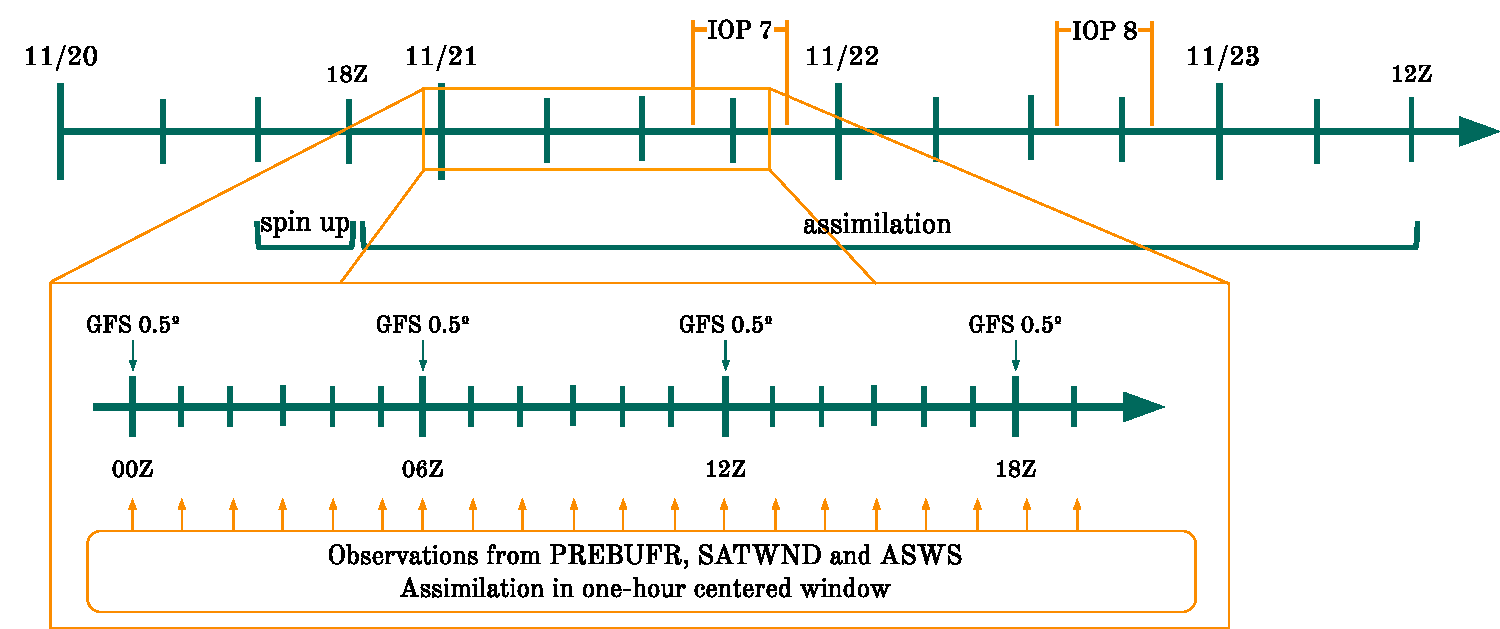
\includegraphics[width=1\linewidth]{../figures/analysis_cycle} \caption{Diagram of the analysis cycles between 18 UTC Nov 20, and 12 UTC Nov 23 plus spin up period of 6 hours. The zoomed section shows the hourly assimilation that is performed within a one-hour centered window and new boundary conditions from GFS every 6 hours. The two IOP missions from the RELAMPAGO field campaign and the ensemble forecast initialized at 00 and 06 UTC Nov 22 are shown.}\label{fig:cycle}
\end{figure}

\hypertarget{verification-methods}{%
\subsection{Verification methods}\label{verification-methods}}

A set of metrics are selected to evaluate different aspects of the analysis obtained in the experiments conducted in this paper. These aspects include a validation of how the uncertainty is quantified in the first-guess and in the analysis, and how different experiments fit an independent set of observations that are not assimilated.

To evaluate the statistical consistency of the uncertainty quantification in the ensemble system the Reduced Centered Random Variable (RCRV, \citet{candille2007}) is used which is defined as:

\begin{equation}
  \mathrm{RCRV = \frac{m - x_o}{\sqrt{\sigma_o^2 + \sigma^2}}}
  \label{eq:eq2}
\end{equation}

where \(x_o\) is the assimilated observation and its error \(\sigma_o\), the ensemble mean of the analysis in observational space \(m\), and the standard deviation \(\sigma\) of the ensemble. The \(RCRV\) is the ratio of the distance between the observations and the forecast and its expected standard deviation assuming the statistical independence between the forecast error (estimated from the ensemble spread) and the observation error. The average of \(RCRV\) computed over all the analysis cycles represents the bias of the ensemble mean with respect to the observations normalized by the estimated uncertainty:

\begin{equation}
  \mathrm{\mathit{mean RCRV} = E[RCRV]}
  \label{eq:eq3}
\end{equation}

If the ensemble has a positive bias, \(mean RCRV\) will be positive, on the opposite, if the ensemble has a negative bias, \(mean RCRV\) will be negative. The standard deviation of the \(RCRV\) or \(sd RCRV\) is defined as:

\begin{equation}
  \mathrm{\mathit{sd RCRV} = \sqrt{\frac{1}{M -1}\sum_{i=1}^{M}(\mathit{RCRV_i} - \mathit{mean RCRV})^2}}
  \label{eq:eq4}
\end{equation}

where \(M\) is the ensemble size. The \(sd RCRV\) measures how large is the distance between the forecast and the observations with respect to the expected distance (given by the combination of the ensemble spread and the observation error). Assuming that the observation error is accurately estimated, an \(sd RCRV > 1\) indicates that the ensemble is underdispersive (i.e.~the distance between the observations and the forecasts is larger than expected), and an \(sd RCRV < 1\) indicates that the ensemble is overdispersive (i.e.~the distance between the observations and the forecasts is lower than expected). A consistent system will have no bias (\(mean RCRV = 0\)) and a standard deviation equal to 1 (\(sd RCRV = 1\)).

The fit of the first-guess and analysis to a set of independent observations, the high-resolution radiosondes from RELAMPAGO, is computed based on the Root Mean Square Error (RMSE) and the BIAS:

\begin{equation}
  \mathrm{\mathit{RMSE} = \sqrt{\frac{1}{N}\sum_{i = 1}^{N} (X_i - O_i)^{2}}}
  \label{eq:eq5}
\end{equation}

\begin{equation}
  \mathrm{\mathit{BIAS} = \frac{1}{N}\sum_{i = 1}^{N} (X_i - O_i)}
  \label{eq:eq6}
\end{equation}

where \(O\) and \(X\) stand for independent observations and the simulations respectively, and N is the sample size.

For the comparison of the first-guess precipitation with the IMERG precipitation estimates, the Fractions Skill Score (FSS, \citet{roberts2008}) is computed for different neighborhood length scales and thresholds:

\begin{equation}
  \mathrm{\mathit{FSS} = 1-\frac{\sum_{i=1}^{N} ({P_x}_i-{P_o}_i)^{2}}{\sum_{i=1}^{N} ({P_x}_i)^{2}+\sum_{i=1}^{N} ({P_o}_i)^{2}}}
  \label{eq:eq7}
\end{equation}

where \(P_{oi}\) is the fraction of grid points in the \(i-th\) sampling area in which the observed accumulated precipitation is greater than a specified threshold. Following \citet{roberts2020}, \(P_{xi}\) is calculated from the ensemble probability precipitation over the same threshold in each grid point by averaging over the \(i-th\) sampling area.
The FSS was computed from the accumulated precipitation over 6 hr rolling windows by adding the 1-hr accumulated precipitation forecasts over 6 consecutive assimilation cycles.

\hypertarget{computation-procedures}{%
\subsection{Computation procedures}\label{computation-procedures}}

All the experiments were performed at the National Center for Atmospheric Research (NCAR) supercomputer Cheyenne \citep{Cheyenne2019}. All the analyses in this paper were conducted using the R programming language \citep{rcoreteam2020}, using data.table \citep{dowle2020} and metR \citep{campitelli2020} packages.
All graphics are made using ggplot2 \citep{wickham2009} and the paper was rendered using knitr and rmarkdown \citep{xie2015, allaire2019}.

\hypertarget{results}{%
\section{Results}\label{results}}

\hypertarget{ensemble-consistency}{%
\subsection{Ensemble consistency}\label{ensemble-consistency}}

To investigate the ability of the first-guess ensemble mean to fit the observations taking into account the uncertainties of the forecast and the observations, the \(mean RCRV\) and the \(sd RCRV\) is calculated for the RAD experiment. As this experiment assimilates all types of observations used in this work, it is possible to analyze the consistency of the ensemble by comparing it with each type of observation. Figure \ref{fig:rcrv-sfc} shows the \(sd RCRV\) for surface observations box-averaged to a 2.5° grid. The \(sd RCRV\) for wind observations (Figure \ref{fig:rcrv-sfc}a) is close to 1 suggesting a good agreement between the ensemble spread, the forecast error, and the observation error. For the temperature (Figure \ref{fig:rcrv-sfc}b), the results are similar except that for some areas in the west of the domain the \(sd RCRV\) can be as high as 4.5. These higher values of \(sdRCRV\) can be associated with systematic errors arising from high differences between the model surface and the observations. Small scale circulations associated with the complex terrain and not well resolved by the model can also contribute to increase the distance between the forecast and the observations. These aspects are usually not captured by the ensemble spread unless a well tuned space dependent inflation scheme is used thus leading to greater sdRCRV values.

Figure \ref{fig:rcrv-profile} shows the mean and standard deviation of the RCRV for the upper-air observations. Figures \ref{fig:rcrv-profile}a-b show the RCRV statistics for soundings (ADPUPA) and aircraft (AIRCAR and AIRCFT). Both ADPUPA and AIRCFT show a generally good agreement between the ensemble spread and the observation error. As sounding observations and their associated errors are known to be reliable, this result indicates that the ensemble has an appropriate spread. AIRCAR presents an irregular profile with \(sd RCRV\) values that suggest that the error for this type of observation is overestimated. ADPUPA and AIRCAR present a \(mean RCRV\) profile near zero at middle and upper levels. At low levels, the meanRCRV profile is positive, showing a cold bias present in the model, a characteristic already studied in \citet{ruiz2010} and \citet{dillon2021}.

Satellite-derived winds observations vary in number depending on the satellite and the level. In Figure \ref{fig:rcrv-profile}c only the \(RCRV\) calculated with at least 100 observations for each satellite and level is included. At low levels, where there are not many observations available, the profiles of \(mean RCRV\) and \(sd RCRV\) show a larger departure from the expected behavior with a negative bias, and a possible overestimation of the observation error. Wind estimations derived from water vapor channels are abundant above 500 hPa where their bias is close to zero. The only exception are the EUMETSAT observations which contribute very little in the region.

The mean RCRV profiles calculated from the radiance observations (Figure \ref{fig:rcrv-profile}d) show almost no bias and the same happens if the \(mean RCRV\) is calculated over each channel of each sensor (not shown). This indicates that the bias correction algorithm works as expected. The \(sd RCRV\) values are less than 1 for all sensors possibly due to an overestimation of the observation errors to reduce the influence of potentially erroneous observations.

Overall, these results indicate that the ensemble spread is consistent with the short-range forecast error and that systematic errors are relatively small for most of the observation types used in this work. Moreover, these results suggest the relaxation-to-prior spread inflation parameter \(\alpha = 0.9\) is adequate for the system.



\begin{figure}
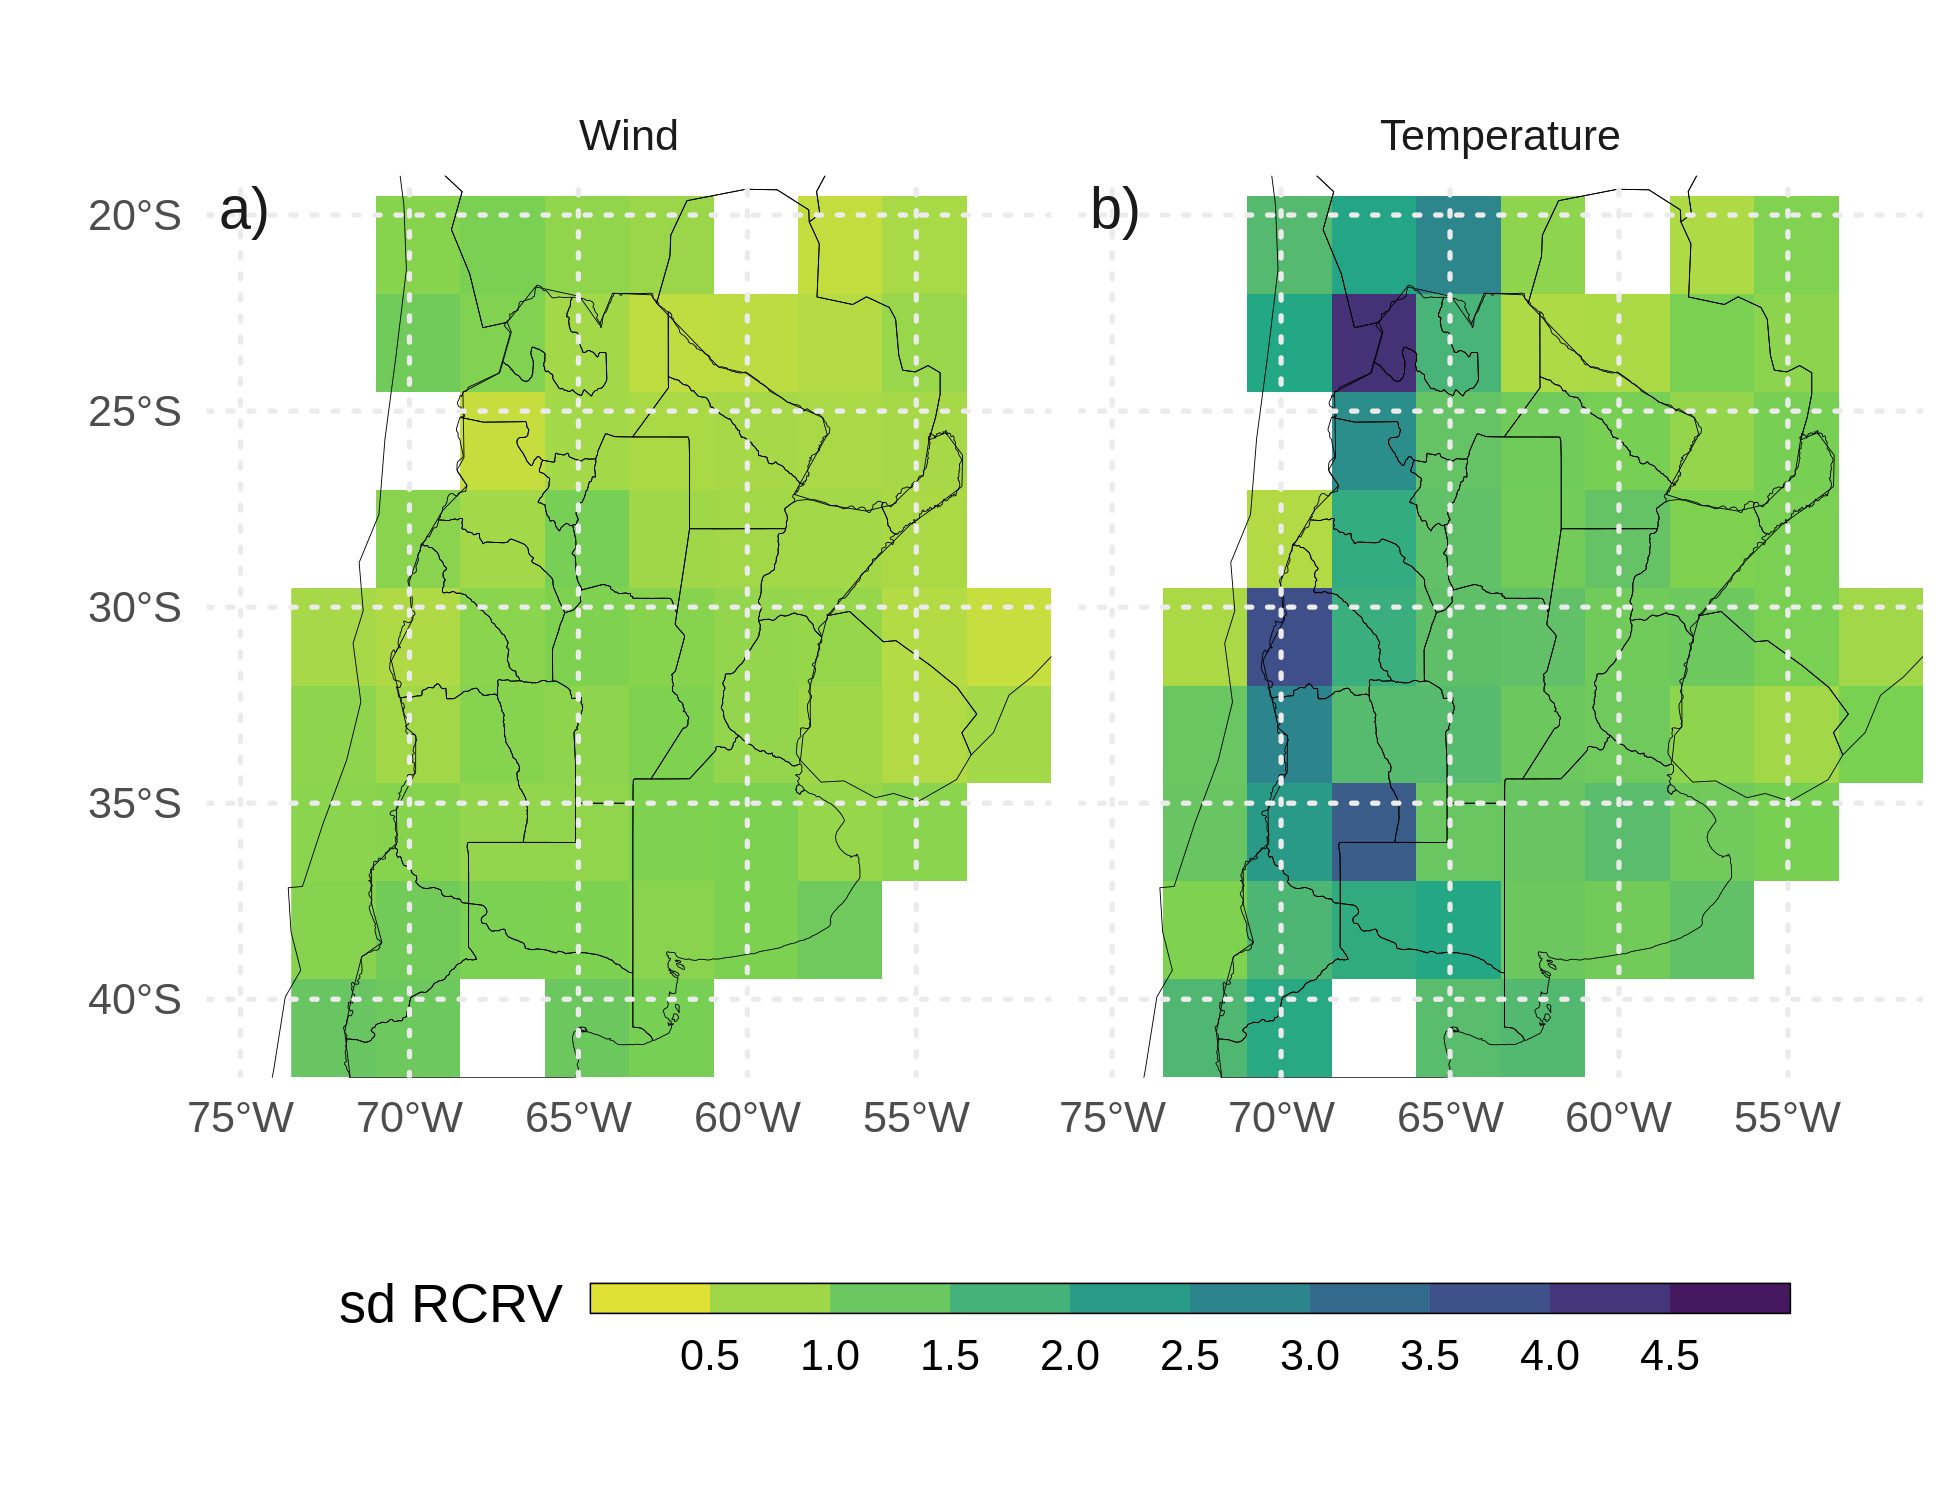
\includegraphics[width=1\linewidth]{../figures/rcrv-sfc-1} \caption{First guess \(sd RCRV\) calculated for surface observations (from PREPBUFR and AWS) of a) wind, and b) temperature averaged over 2.5º boxes for the RAD experiment. Observations were aggregated every hourly cycle for the entire experiment period.}\label{fig:rcrv-sfc}
\end{figure}



\begin{figure*}
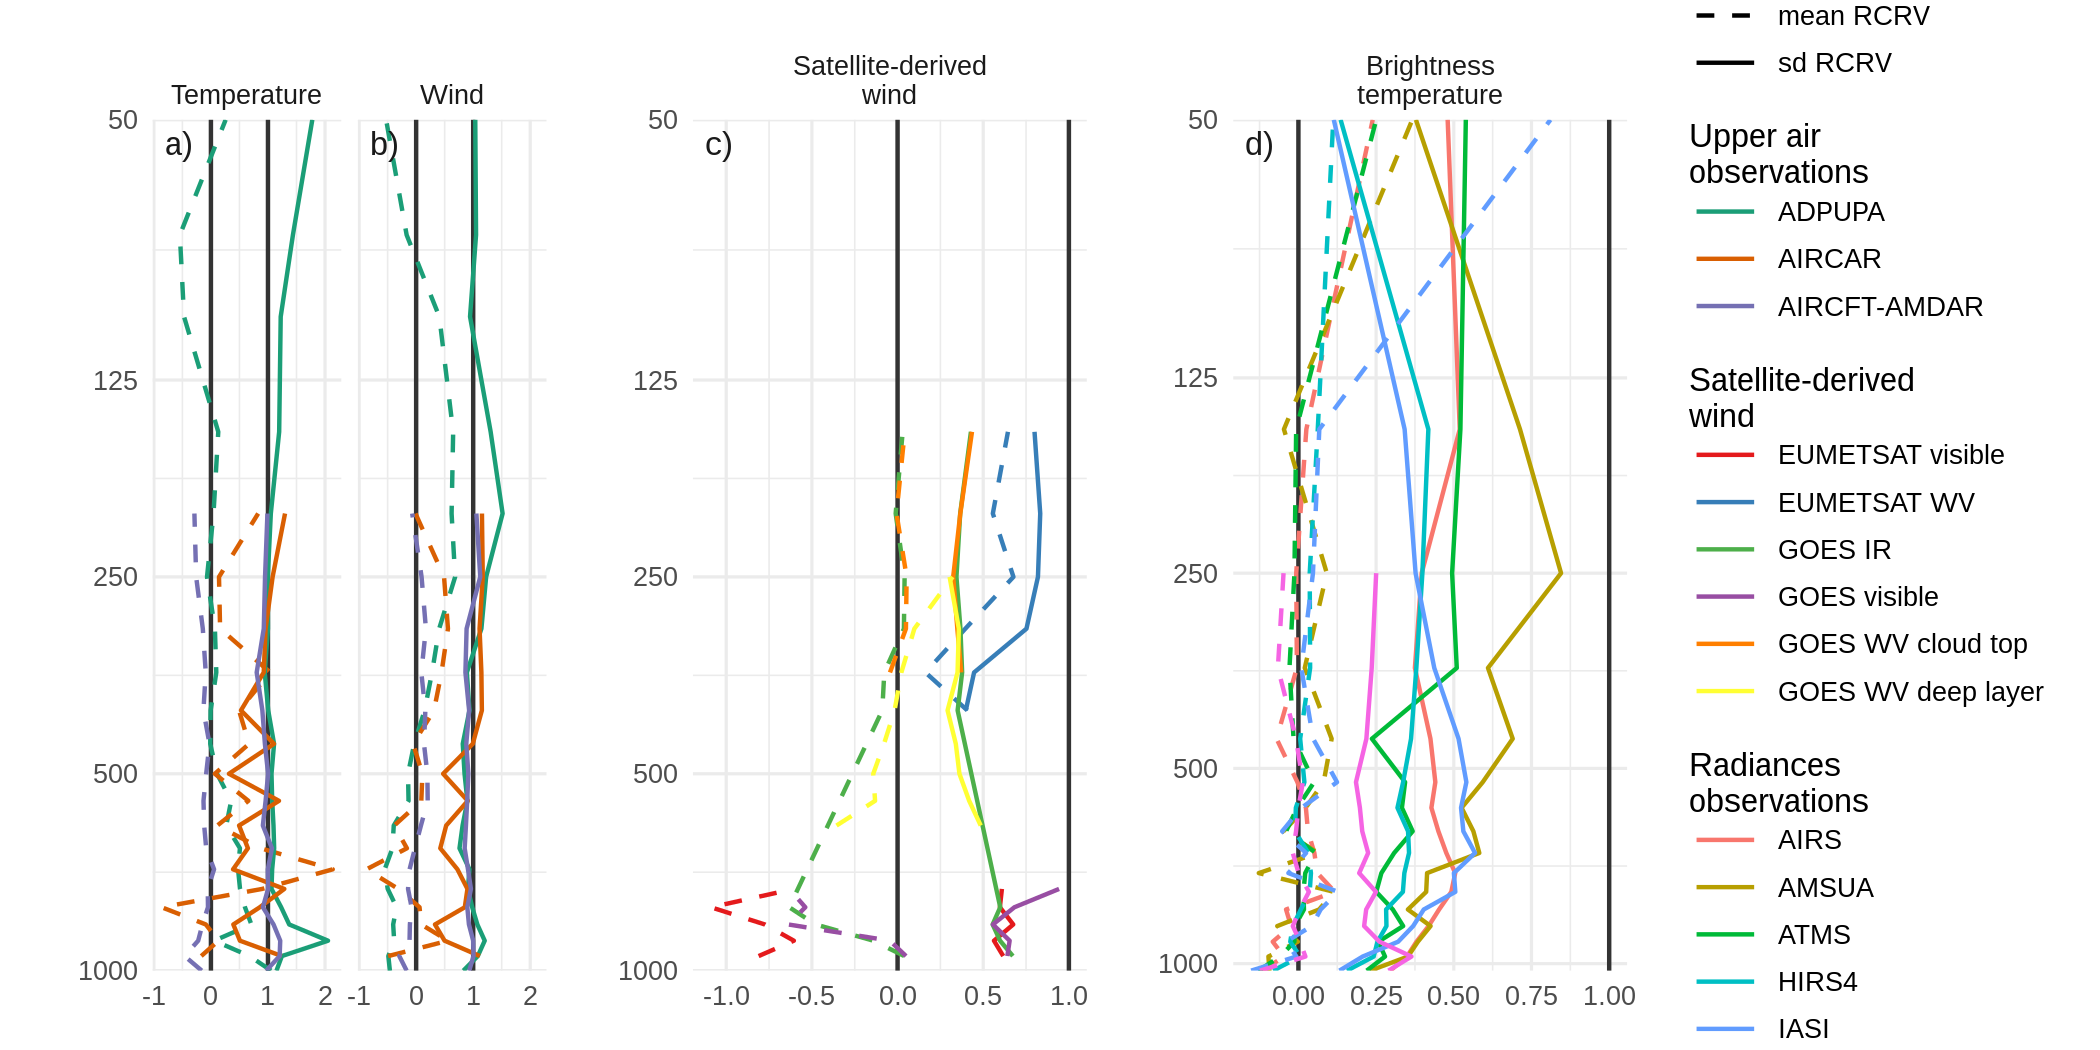
\includegraphics{../figures/rcrv-profile-1} \caption{Vertical profiles of first guess \(mean RCRV\) (dashed line) and \(sd RCRV\) (solid line) for a) temperature and b) wind of sounding and aircraft observations, c) satellite-derived wind observations, and d) brightness temperature observations for the RAD experiment. Observations were aggregated every hourly cycle for the entire experiment period.}\label{fig:rcrv-profile}
\end{figure*}

\hypertarget{impacts-of-assimilated-observations}{%
\subsection{Impacts of assimilated observations}\label{impacts-of-assimilated-observations}}

This section presents the impact of assimilating different observation types on variables which are particularly relevant for the occurrence of deep moist convection. The analysis is performed over a smaller domain (red box in Figure \ref{fig:dominio}a) to focus on the region most directly affected by the MCS. Figures \ref{fig:TQ-diff}a-c show the analysis difference between experiments in the spatially averaged vertical profile of temperature. By averaging the differences between two experiments the systematic impact produced by different observing systems on the analyzed state can be isolated. During the first day, the assimilation of AWS observations results in a colder PBL. This cooling effect has a clear diurnal cycle, being stronger during nighttime (Figure \ref{fig:TQ-diff}a). During the second day of the experiment, the impact of AWS observations extends into the middle and upper troposphere coinciding with the mature stage of the MCS. The warm difference shown in AWS-CONV between 500 and 200 hPa is produced by the development of stronger convection in AWS compared to CONV. This is a good example of how low-level information provided by surface weather stations can rapidly spread into the troposphere in the presence of deep moist convection. Although the mid-to-upper circulation can have an important impact on the organization and evolution of the MCS over the region, the satellite-derived winds did not have an appreciable impact on the mean temperature and humidity (Figure \ref{fig:TQ-diff}b-e), possibly due to the large observation errors used for the assimilation.
During the first day of the experiment, the assimilation of radiances produces a warming effect in the PBL which partially compensates for the cooling effect of AWS observations (Figure \ref{fig:TQ-diff}c). No clear systematic impact is found above the PBL during this period. During the second day, the impact of radiance observations is found through the troposphere with a distribution that is similar to the impact found in the AWS experiment but with the opposite sign.

Comparing the specific humidity in the experiments (Figures \ref{fig:TQ-diff}d-f), the impact of assimilating AWS with fine spatial and temporal resolution is most substantial at low levels (Figure \ref{fig:TQ-diff}d). The PBL in the AWS experiment is consistently moister than in the CONV experiment, particularly at nighttime. The increase in low-level moisture by a denser surface network is consistent with previously reported dry biases in the WRF model over the region \citep[\citet{matsudo2021}, \citet{ruiz2010}]{casaretto2022}. The moistening of the PBL is mainly driven by the covariance between temperature and specific humidity within the PBL. In the experiment and over the center of the domain, this covariance remains negative, increasing low-level moisture as the observations introduce negative temperature corrections. As for the temperature, the systematic impact of satellite-derived winds on moisture is small (Figure \ref{fig:TQ-diff}e). Figure \ref{fig:TQ-diff}f shows that radiances reduce low-middle level moisture during the first day of the experiment. The drying effect extends to lower-middle levels during the second day of the experiment coinciding with the development of the MCS between 00 and 12 UTC Nov 22.



\begin{figure*}[ht]

{\centering 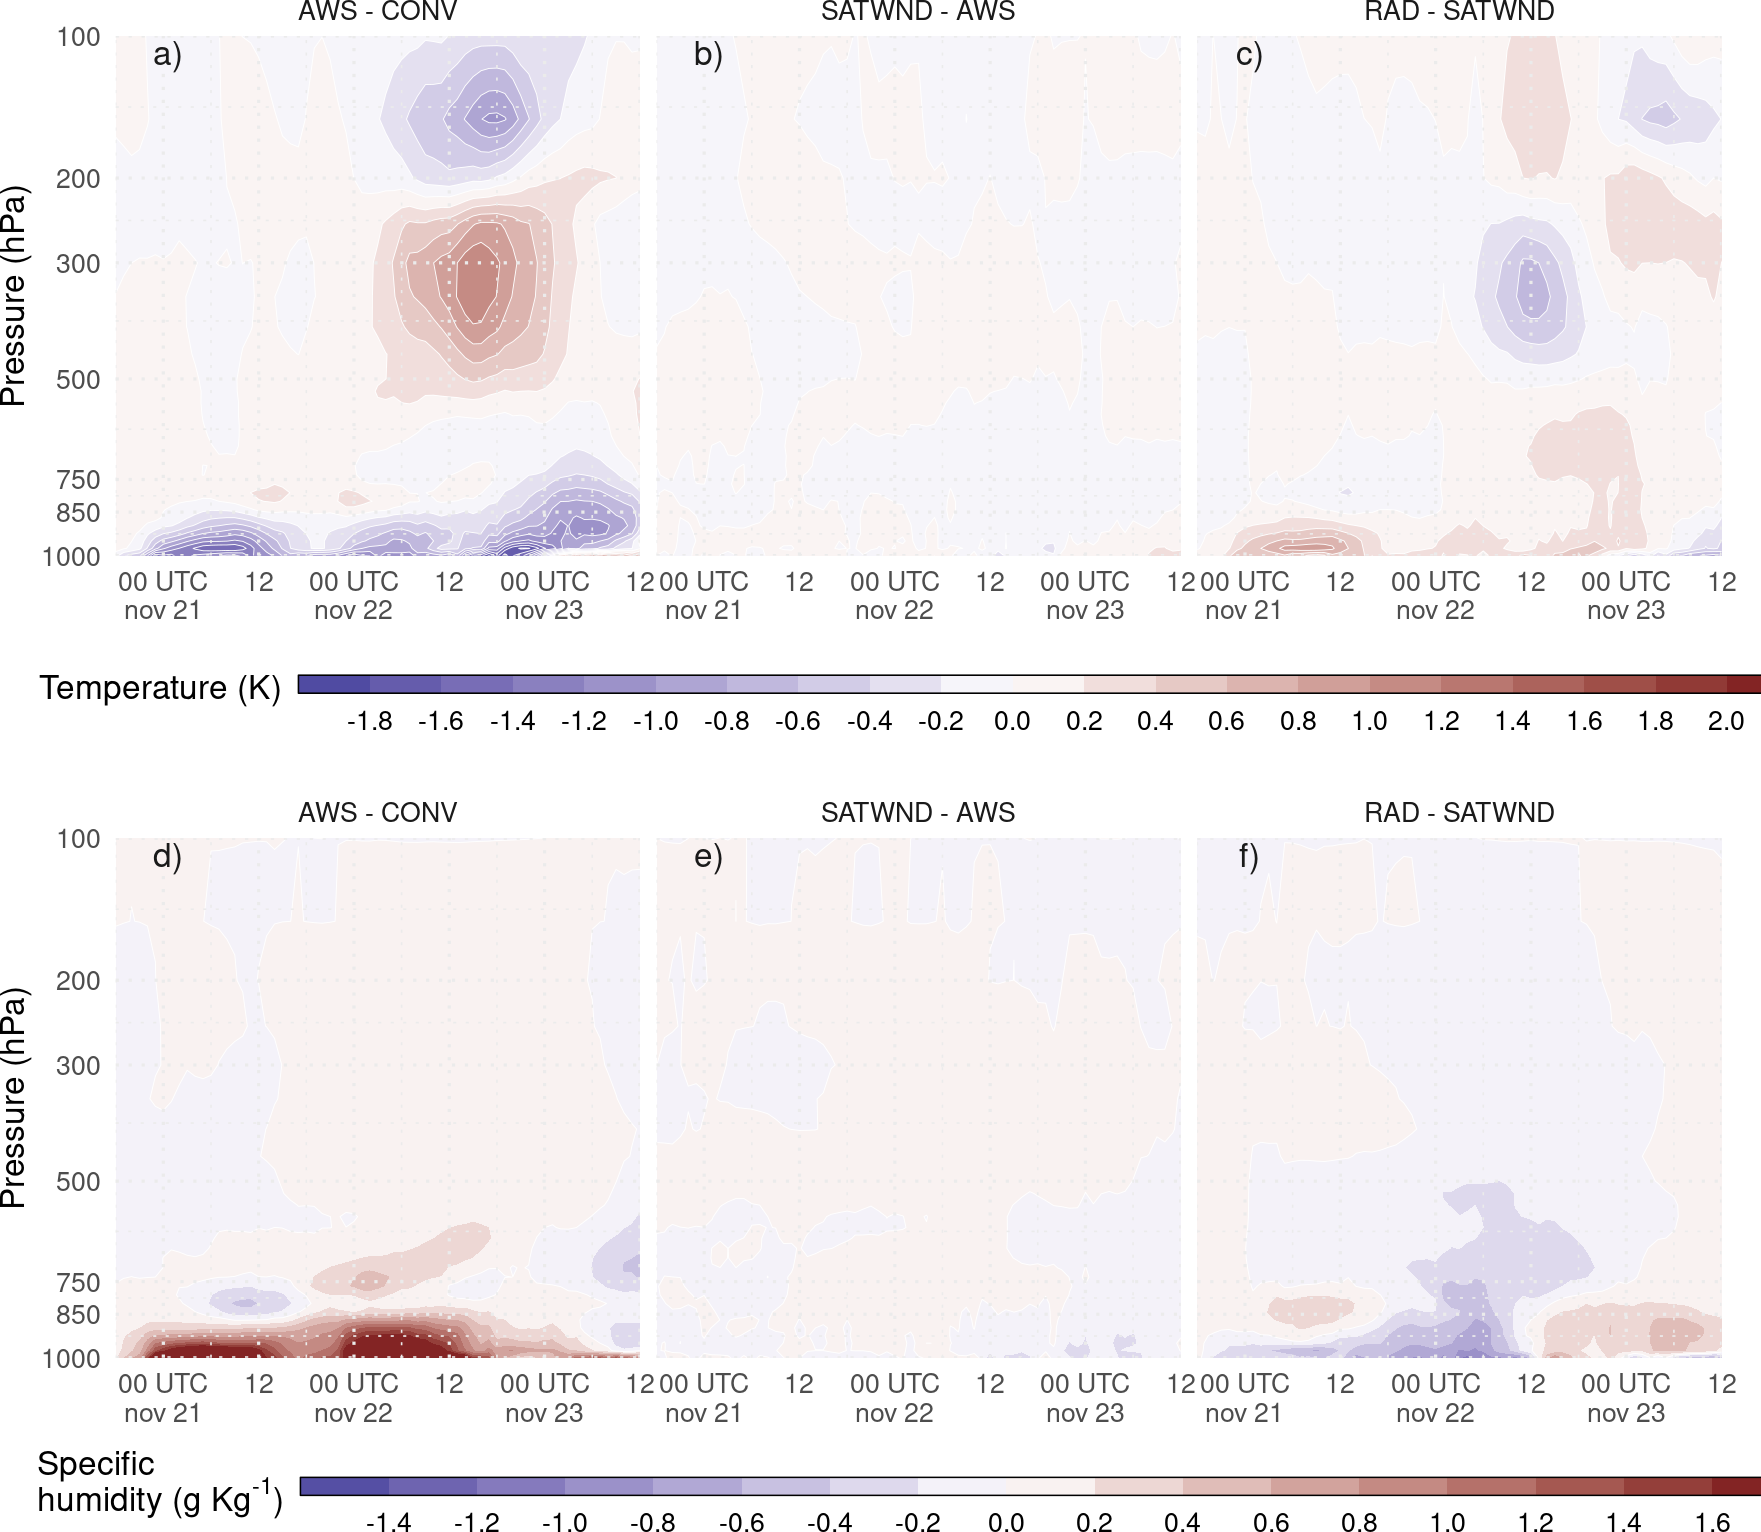
\includegraphics{../figures/TQ-diff-1} 

}

\caption{Difference between analysis ensemble mean experiments a) and d) AWS-CONV, b) and e) SATWND-AWS, and c) and f) RAD-SATWND for the spatially averaged vertical profiles of temperature (a, b, and c, in \(K\)) and specific humidity (d, e, and f in \(g\ kg^{-1}\)) calculated over the inner domain (red box in Figure \ref{fig:dominio}a) for each analysis cycle.}\label{fig:TQ-diff}
\end{figure*}

The impacts on the wind components are shown in Figure \ref{fig:UV-diff}, along with the corresponding averaged wind component in the experiment with the largest number of assimilated observations (for example, Figure \ref{fig:UV-diff}a shows the zonal wind difference between AWS and CONV and the zonal wind for AWS). The assimilation of AWS produces a more easterly wind and a less northerly wind at low levels during the first two days of analysis (Figures \ref{fig:UV-diff}a,b). There is a diurnal cycle in the impact of surface weather stations on the meridional velocity (Figure \ref{fig:UV-diff}d) with a stronger reduction of the northerly wind during night hours. This indicates that surface observations are reducing the intensity of the low level jet present in the pre-convective environment. After 18 UTC Nov 22, the opposite effect is observed when the MCS is moving through the domain to the northeast. After the initiation of the convective cells, the systematic impact on the wind field is larger at mid and upper levels (Figures \ref{fig:UV-diff}d, f). During Nov 22 and 23 the impact of assimilating AWS observations produces an increase of northerly wind in upper levels. This could be a consequence of a stronger MCS with an increased polar side upper level outflow. Although satellite-derived wind observations produce the largest impact in mid-to-upper levels where the number of observations is largest; the systematic impact is overall smaller than the one produced by assimilating data from AWS (Figures \ref{fig:UV-diff}b, e). The reason of the small impact observed in SATWND could be associated to the large observation error used for satellite-derived wind observations.

The assimilation of radiances produces a reduction in the westerly wind compared with respect to SATWIND in low and upper levels (Figure \ref{fig:UV-diff}c). For the meridional wind, these observations produce an enhancement on average of the northerly low-level flow of \(1 ms^{-1}\), opposite to what is generated by the assimilation of AWS observations during the nights, between 03 and 12 UTC, previous to the development of the MCS (Figure \ref{fig:UV-diff}f). At upper levels and during Nov 22 and 23 the average impact of assimilating radiances is a decrease in the wind speed. The meridional wind field at 200 hPa at different times shows that the outflow from the MCS is even more intense than in the other experiments, while the southerly wind ahead of the MCS also increases producing an average reduction of the northerly wind (Figure \ref{fig:UV-diff}f).



\begin{figure*}[ht]

{\centering 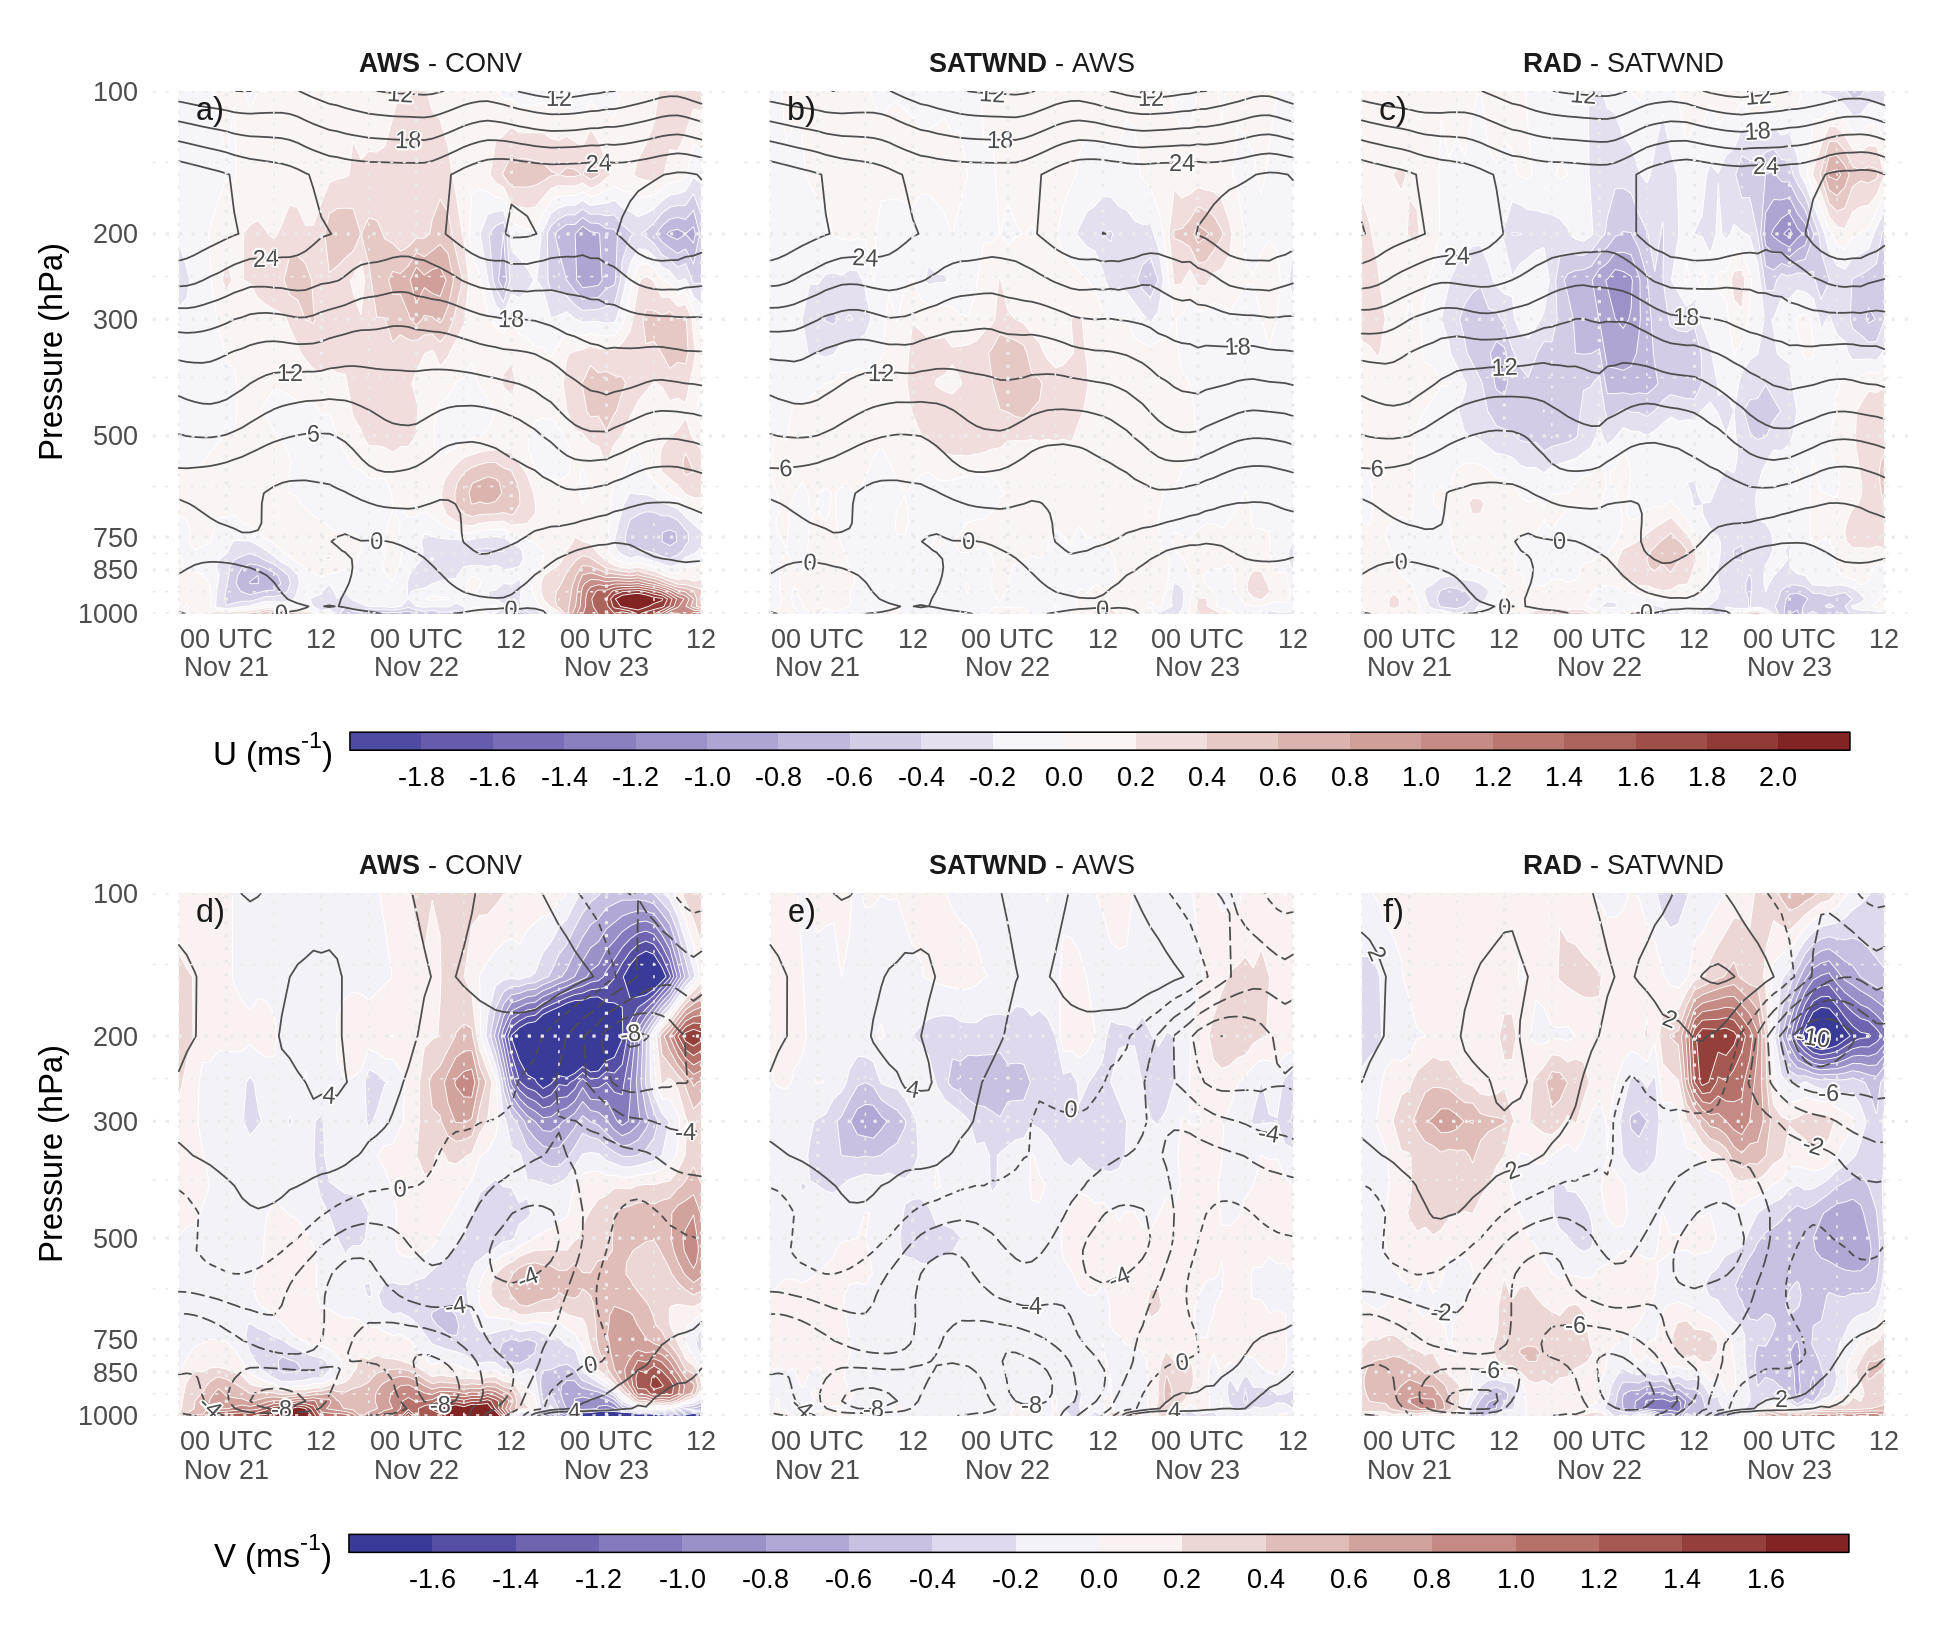
\includegraphics{../figures/UV-diff-1} 

}

\caption{Difference between analysis ensemble mean experiments a) and d) AWS-CONV, b) and e) SATWND-AWS, and c) and f) RAD-SATWND for the spatially averaged vertical profiles of u wind (a, b, and c, in \(m\ s^{-1}\)) and v wind (d, e, and f in \(m\ s^{-1}\)) calculated over the inner domain (red box in Figure \ref{fig:dominio}a) for each analysis cycle. Black contours correspond to u wind and dashed contours to negative v wind for (a) AWS, (b) SATWND, and (c) RAD and v wind for (d) AWS, (e) SATWND, and (f) RAD since those experiments are the ones with more assimilated observations in each panel.}\label{fig:UV-diff}
\end{figure*}

The difference between ERA5 reanalyses \citep[`]{era5pressure} and the ensemble mean analyses are also compared in Figure \ref{fig:era5}, which supports Figures \ref{fig:TQ-diff} and \ref{fig:UV-diff}. Specifically, Figure \ref{fig:era5}a shows a warm bias in low levels (i.e.~CONV is warmer than ERA5) that decreases in Figure \ref{fig:era5}b when the AWS observations are assimilated. In the same direction, Figure \ref{fig:TQ-diff}a shows a negative difference between AWS and CONV meaning that the AWS observations are cooling the low levels. Comparing ERA5-RAD (Figure \ref{fig:era5}d), there is a small increase in the warm bias, associated with the warming produced by the radiance observations as shown in Figure \ref{fig:TQ-diff}c.~A similar effect can be observed for specific humidity, AWS observations partially correct the dry bias present in Figure \ref{fig:era5}e and the assimilation of radiance observations reduces the positive impact of AWS. The impact on the wind components is minor so only the meridional wind is included in Figures \ref{fig:era5}i-l, which show that the radiance observations are mainly responsible for the positive impact observed in the analysis by reducing the distance ERA5-RAD, particularly during the mature stage of the MCS. Overall, the adjustments due to assimilating radiance and AWS observations lead to an ensemble mean analyses closer to ERA5 reanalyses.



\begin{figure*}[ht]

{\centering 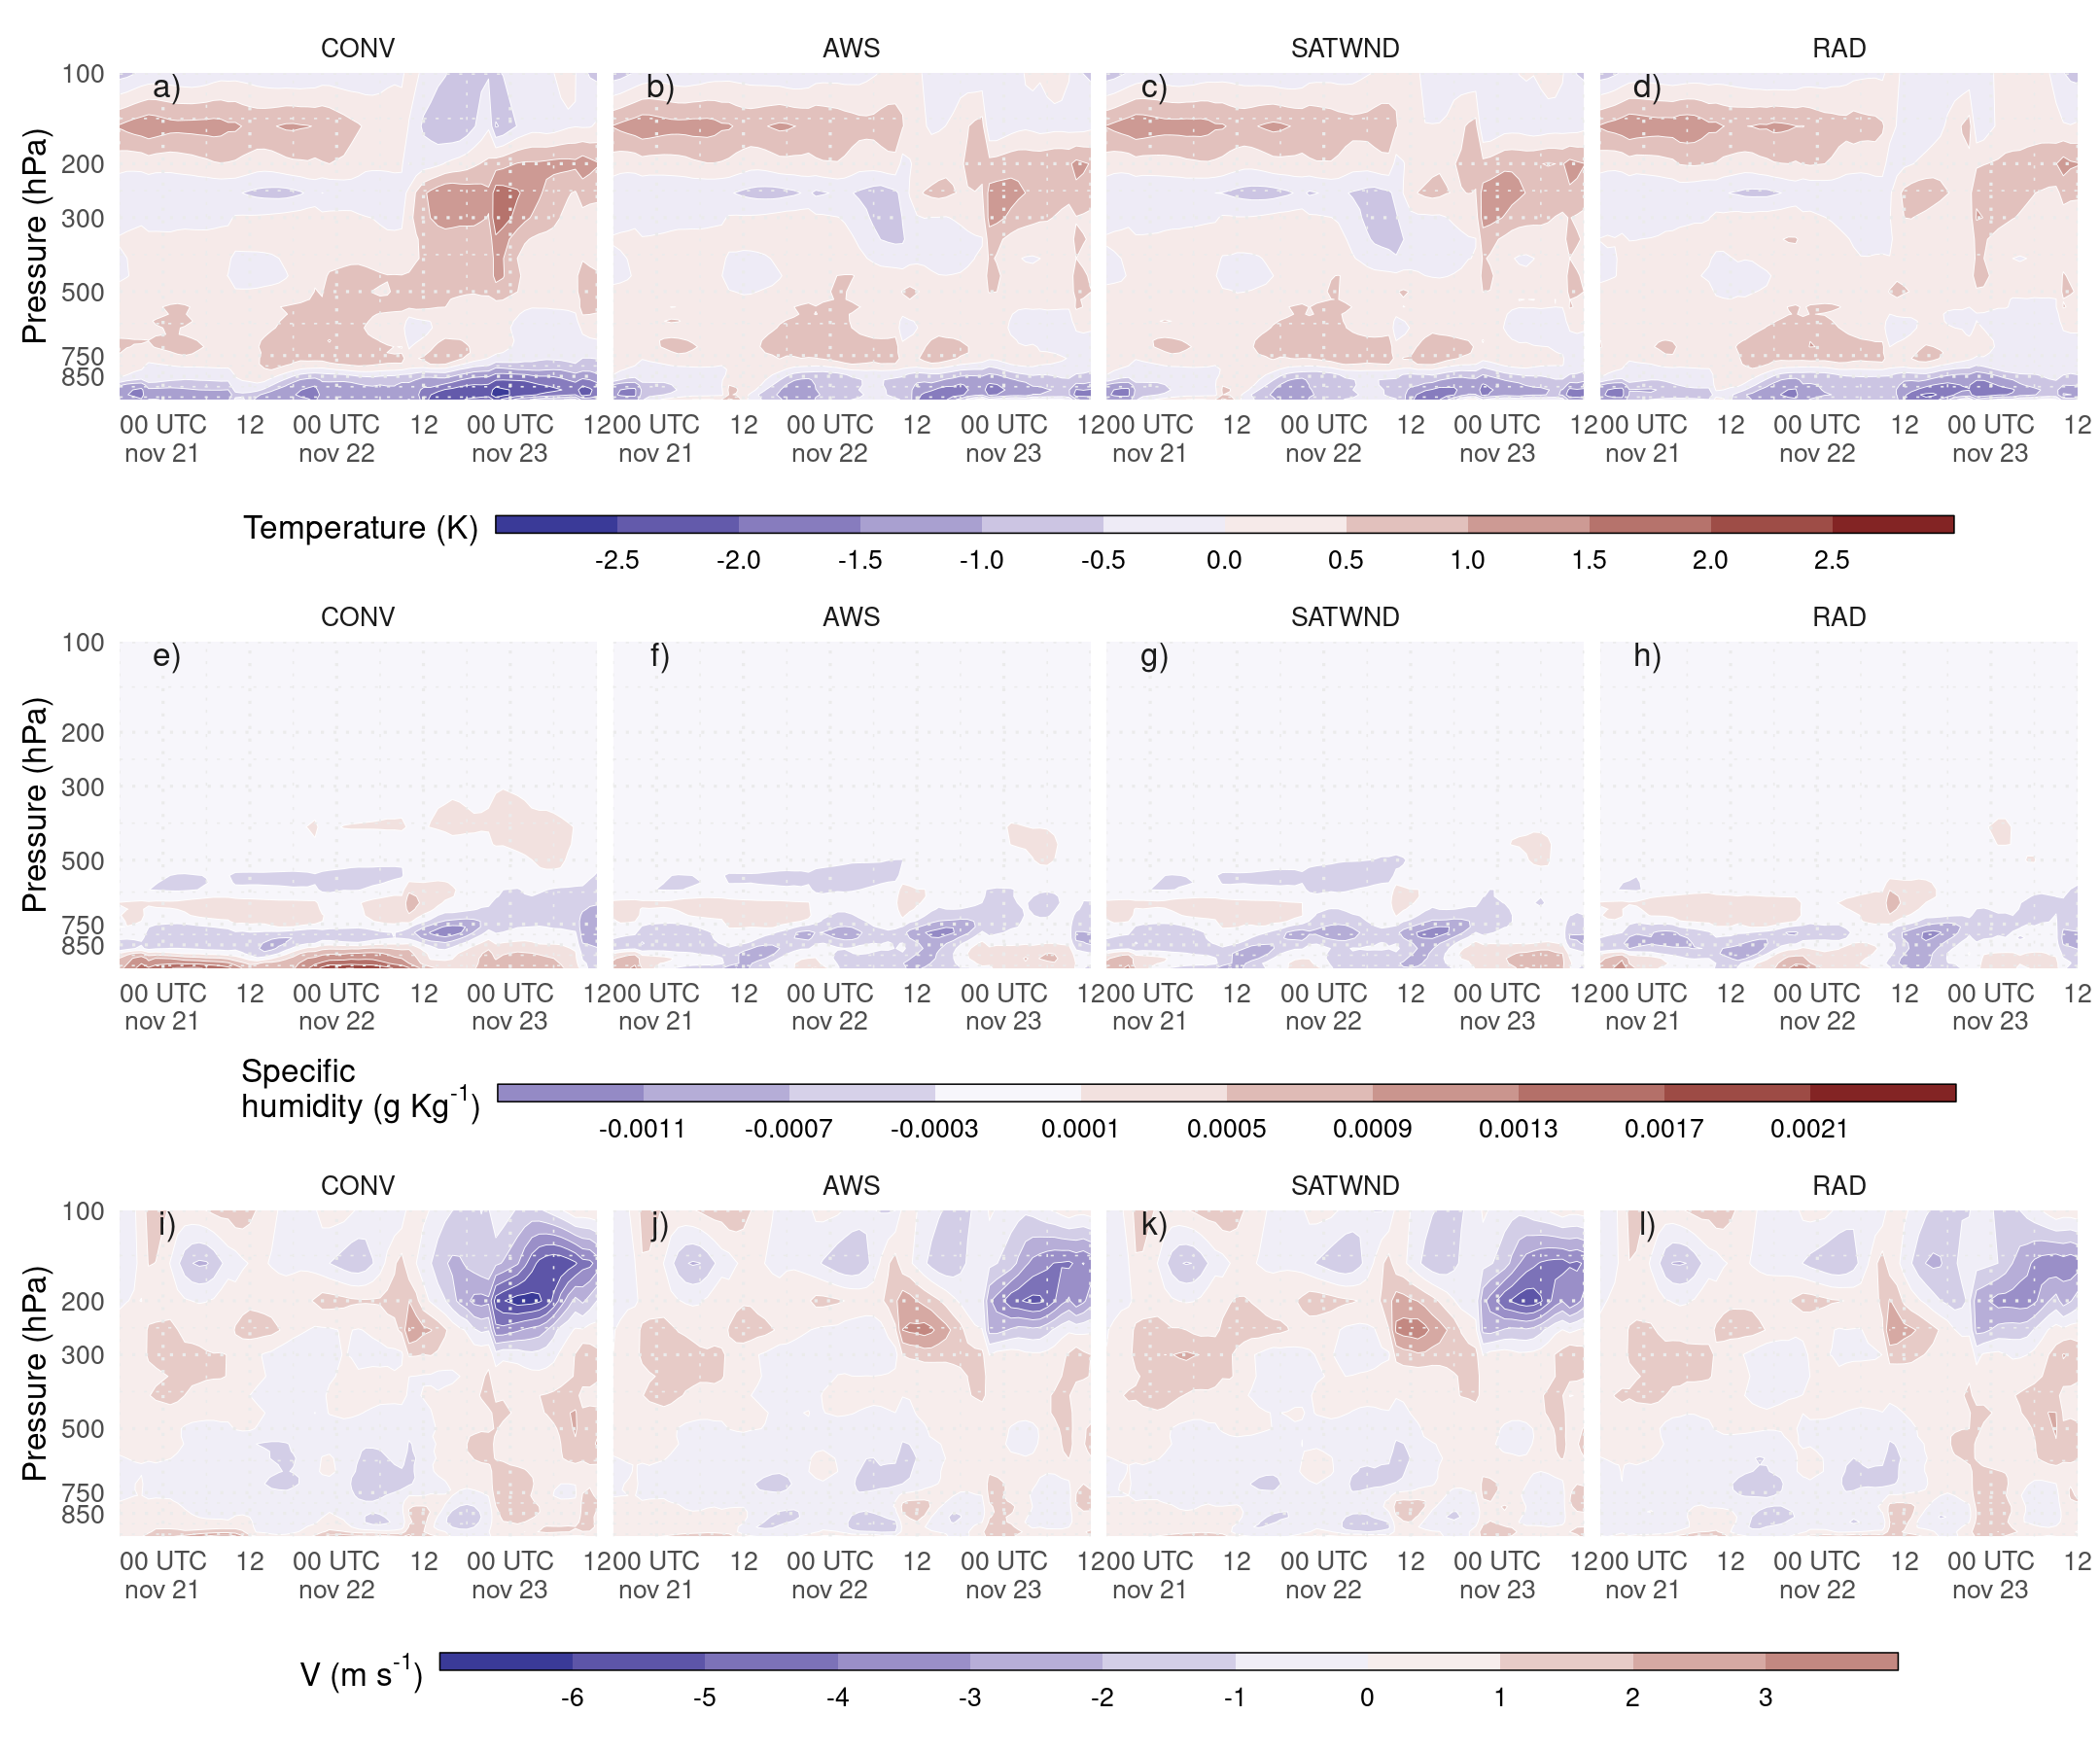
\includegraphics{../figures/era5-1} 

}

\caption{Difference between ERA5 and the analysis ensemble mean experiments for the spatially averaged vertical profiles of air temperature (K, a--d), specific humidity (\(g\ Kg^{-1}\), e--h) and meridional wind (\(m\ s^{-1}\), i--l) calculated over the inner domain (red box in Figure \ref{fig:dominio}a) for each analysis cycle.}\label{fig:era5}
\end{figure*}

To investigate how changes in the PBL can modify the pre-convective environment, the analysis mean horizontal distribution of the low level northerly flow (for the first 7 sigma levels), precipitable water, low level temperature, and CAPE are compared. At 00 UTC Nov 22 (after 30 assimilation cycles) the first convective cells were developing over the southern region of the domain along the cold front. Figure \ref{fig:summary-fields}a shows the precipitable water (shaded) and the vertically averaged low-level meridional wind component (contours). It shows that the moist tongue extending over the northern part of the domain is enhanced by the assimilation of denser surface observations. The moisture increase is particularly strong at the southern tip of this tongue, just ahead of the cold front where convection initiation was taking place. AWS and SATWND experiments are very similar, with values of precipitable water over 55 \(kgm^{-2}\) north of 30\(^{\circ}\)S and a similar vertical distribution of specific humidity (not shown). RAD has lower precipitable water content than AWS and SATWND, but higher than CONV. The distribution of moisture at low levels in RAD seems to be the result of the combination of the moistening effect of assimilating AWS -- partially compensated by the assimilation of radiance observations -- and a reduced meridional moisture transport due to the weaker northerly flow over the center of the domain compared to CONV.

The analyzed distribution of temperature and moisture in the PBL (Figure \ref{fig:summary-fields}b) resembles the characteristics observed in the temperature profiles (Figure \ref{fig:TQ-diff}a-c) where AWS produces a colder PBL than CONV while the PBL in RAD is warmer than in SATWND. On average the PBL in AWS and SATWND is colder than in CONV, while RAD shows a warmer PBL than AWS due to the assimilation of radiance observations. A warmer PBL increases the potential instability and helps to generate a suitable environment for the development of deep convection. Figure \ref{fig:summary-fields}c shows the most unstable convective available potential energy (MCAPE, shaded) and the 0 to 6 \(km\) wind shear. The values of MCAPE in CONV do not exceed 2000 \(J\ Kg^{-1}\) while the rest of the experiments show maximum MCAPE over 4000 \(J\ Kg^{-1}\). MCAPE in the RAD experiment is lower compared to AWS or SATWND. This is consistent with less humidity in the PBL with respect to these experiments but may be partially compensated by a slightly warmer PBL in the RAD experiment. The 0-6 km wind shear is more intense in AWS, SATWND, and RAD reaching values over 15 \(m\ s^{-1}\) at the southern tip of the region with positive MCAPE values. Moreover, in this same region, these experiments show larger MCAPE values than CONV. Note that wind shear over 15 \(m\ s^{-1}\) is associated with the development of more intense and organized MCSs \citep{chen2015} and also with conditions favorable for supercells \citep{markowski2010}.



\begin{figure*}
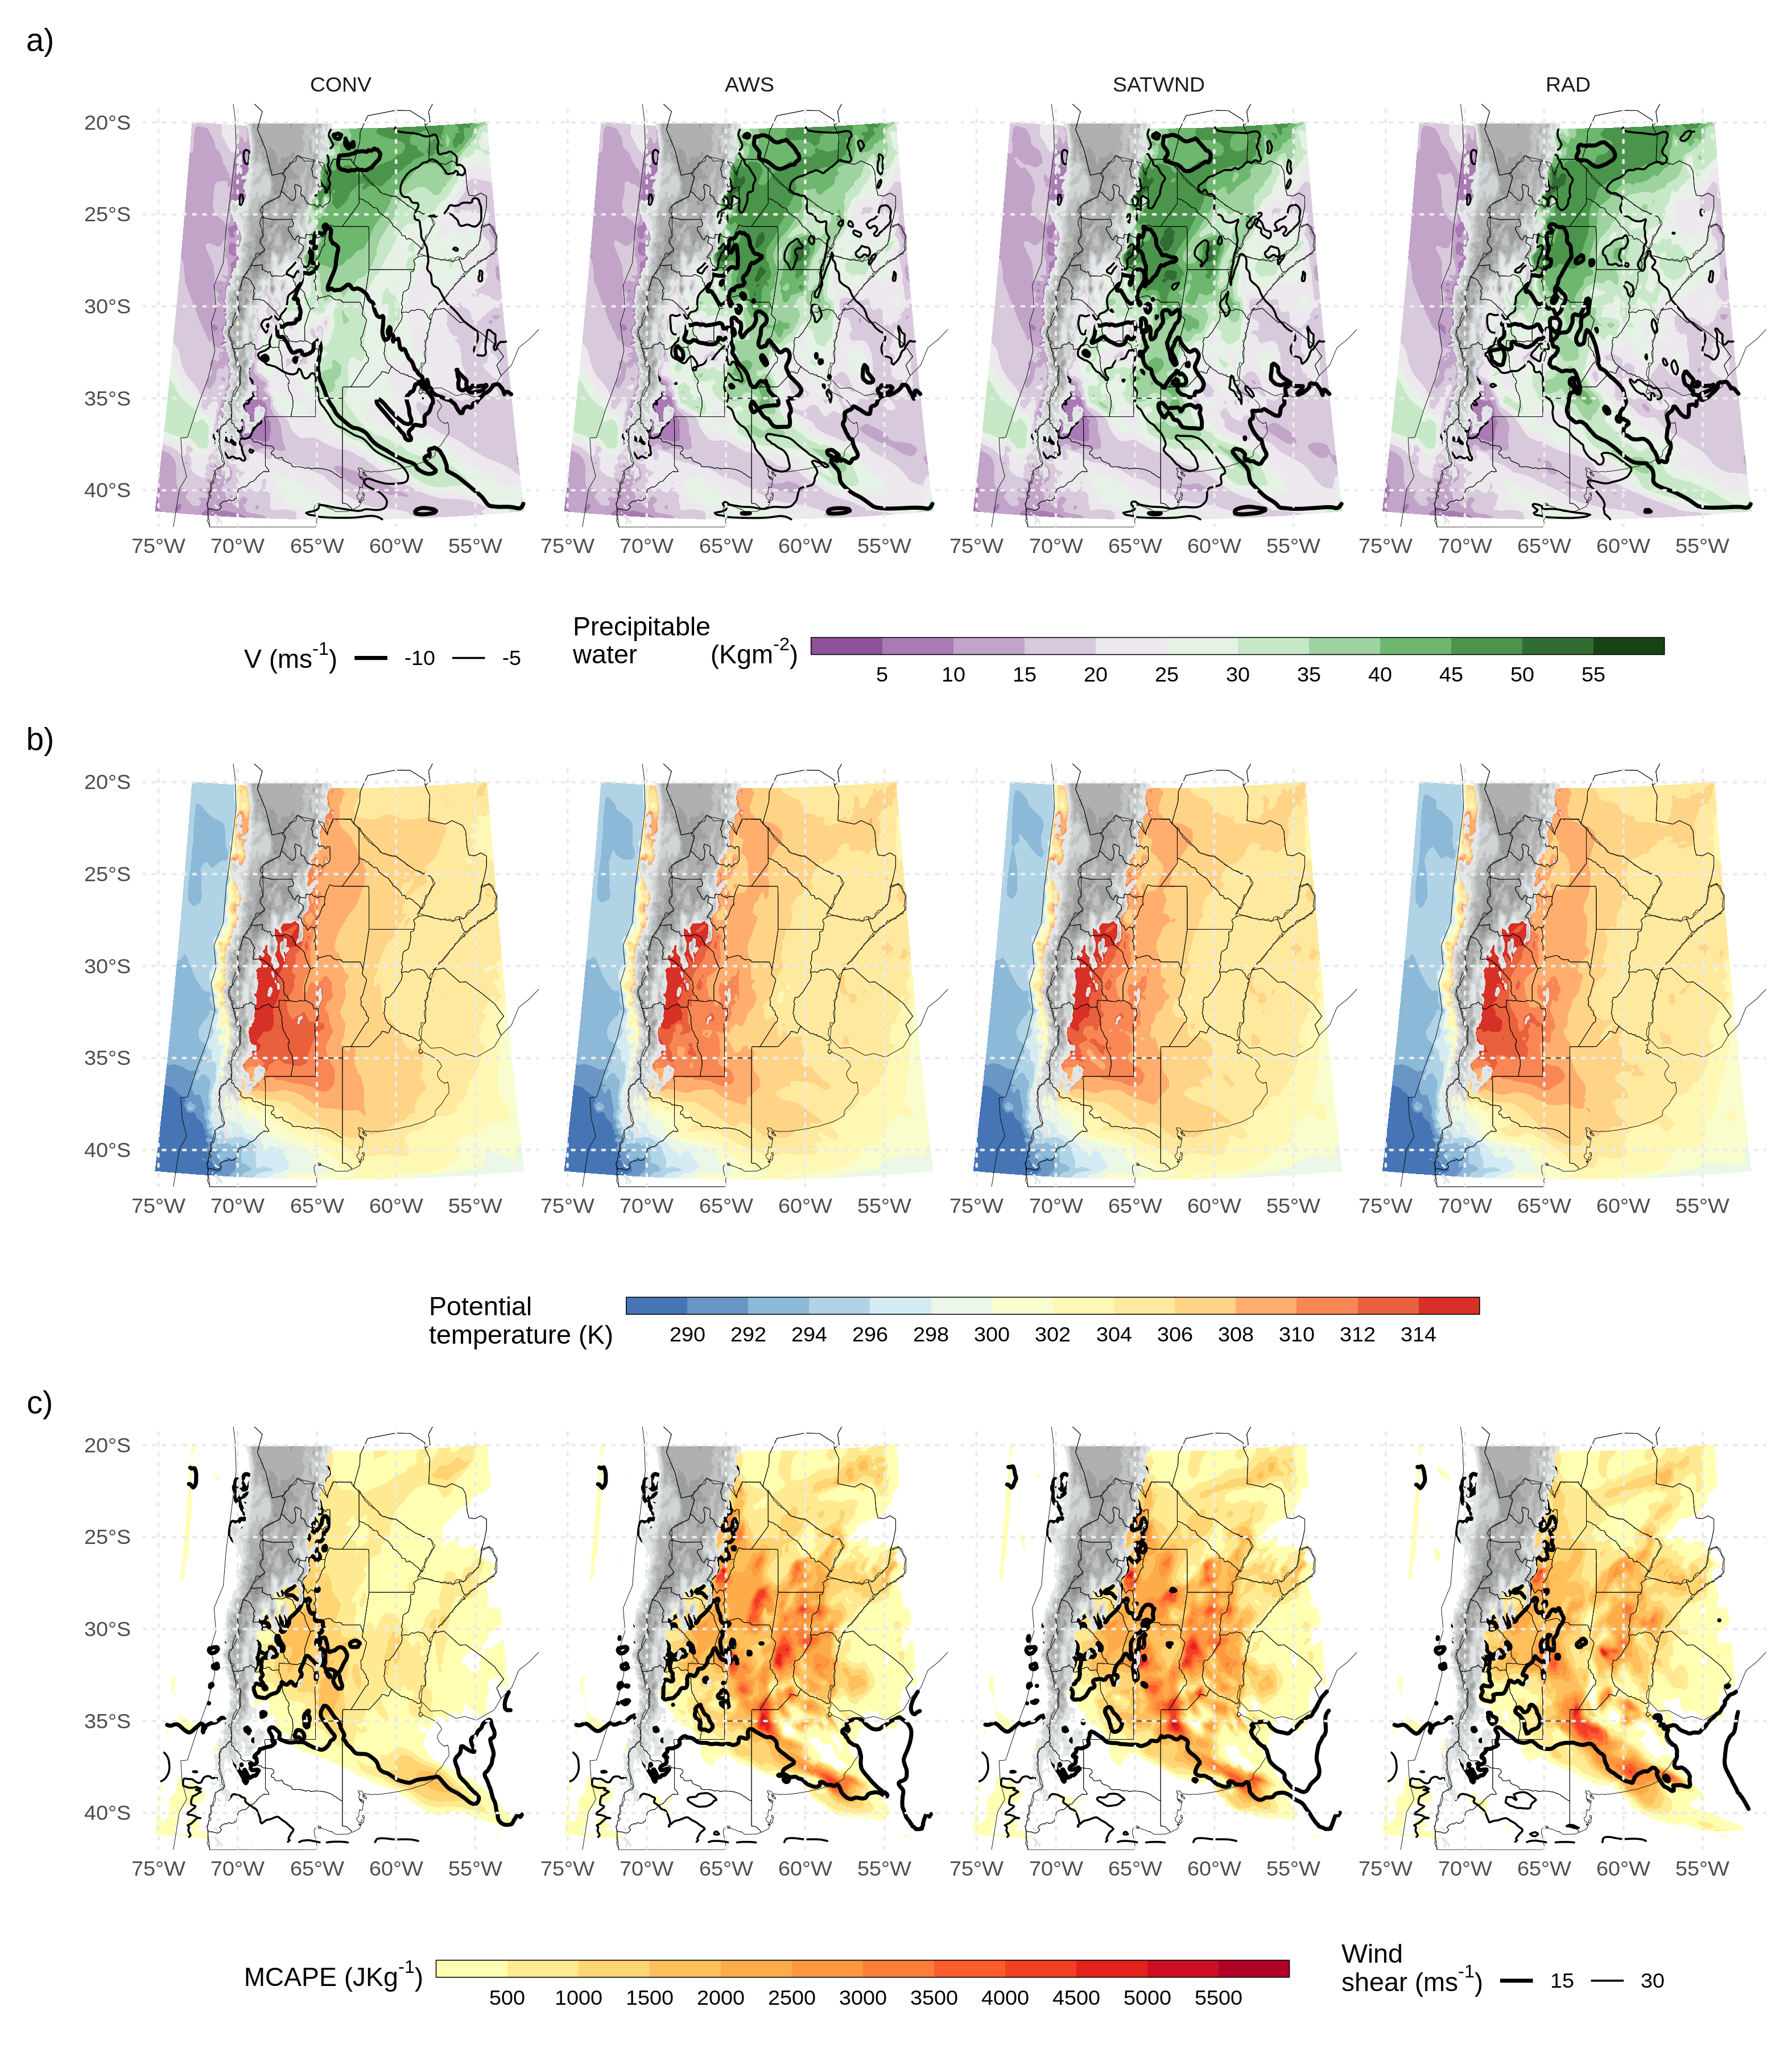
\includegraphics[width=1\linewidth]{../figures/summary-fields-1} \caption{a) Precipitable water (shaded, \(kg\ m^{-2}\)) and average northerly wind over the first 7 sigma levels (from the surface up to approximately 800 hPa, contours, \(m\ s^{-1}\)), b) Average potential temperature for the PBL (first 10 sigma levels), and c) Maximum CAPE and \textasciitilde0-6 km wind shear over 15 and 30 \(m\ s^{-1}\) for each experiment. All fields correspond to the analysis ensemble mean for 00 UTC Nov 22. Grey filled contours correspond to topography over 1500 meters above sea level.}\label{fig:summary-fields}
\end{figure*}

\hypertarget{validation-against-independent-observations}{%
\subsection{Validation against independent observations}\label{validation-against-independent-observations}}

First, the impact of assimilating different observation types in terms of the representation of the MCS and its associated precipitation is analyzed. Figure \ref{fig:pp-hov}a shows the hourly accumulated precipitation as estimated by IMERG, and the probability matched mean (PM) \citep{clark2017} for the first-guess hourly accumulated precipitation as averaged between 67\(^{\circ}\)W and 54.5\(^{\circ}\)W as a function of time and latitude in the different experiments. The heaviest precipitation (over 12 \(mmh^{-1}\)) starts during the afternoon of Nov 22 and continues during Nov 23 after the end of the simulated period (Figure \ref{fig:pp-hov}a). In all the experiments, the accumulated precipitation in the short-range forecasts is underestimated. This is particularly evident in CONV (Figure \ref{fig:pp-hov}b), where the convection initiation is delayed and occurs further north with respect to the observed initiation. AWS, SATWND, and RAD better capture the timing and location of convective initiation (Figures \ref{fig:pp-hov}c-e). AWS and RAD show a more fragmented distribution compared with SATWND, possibly due to the development of less organized convection during Nov 22. After 18 UTC Nov 22, RAD shows improvements in the precipitation rate and its distribution compared to the other experiments as a result of enhanced development of the convection.



\begin{figure*}[h]

{\centering 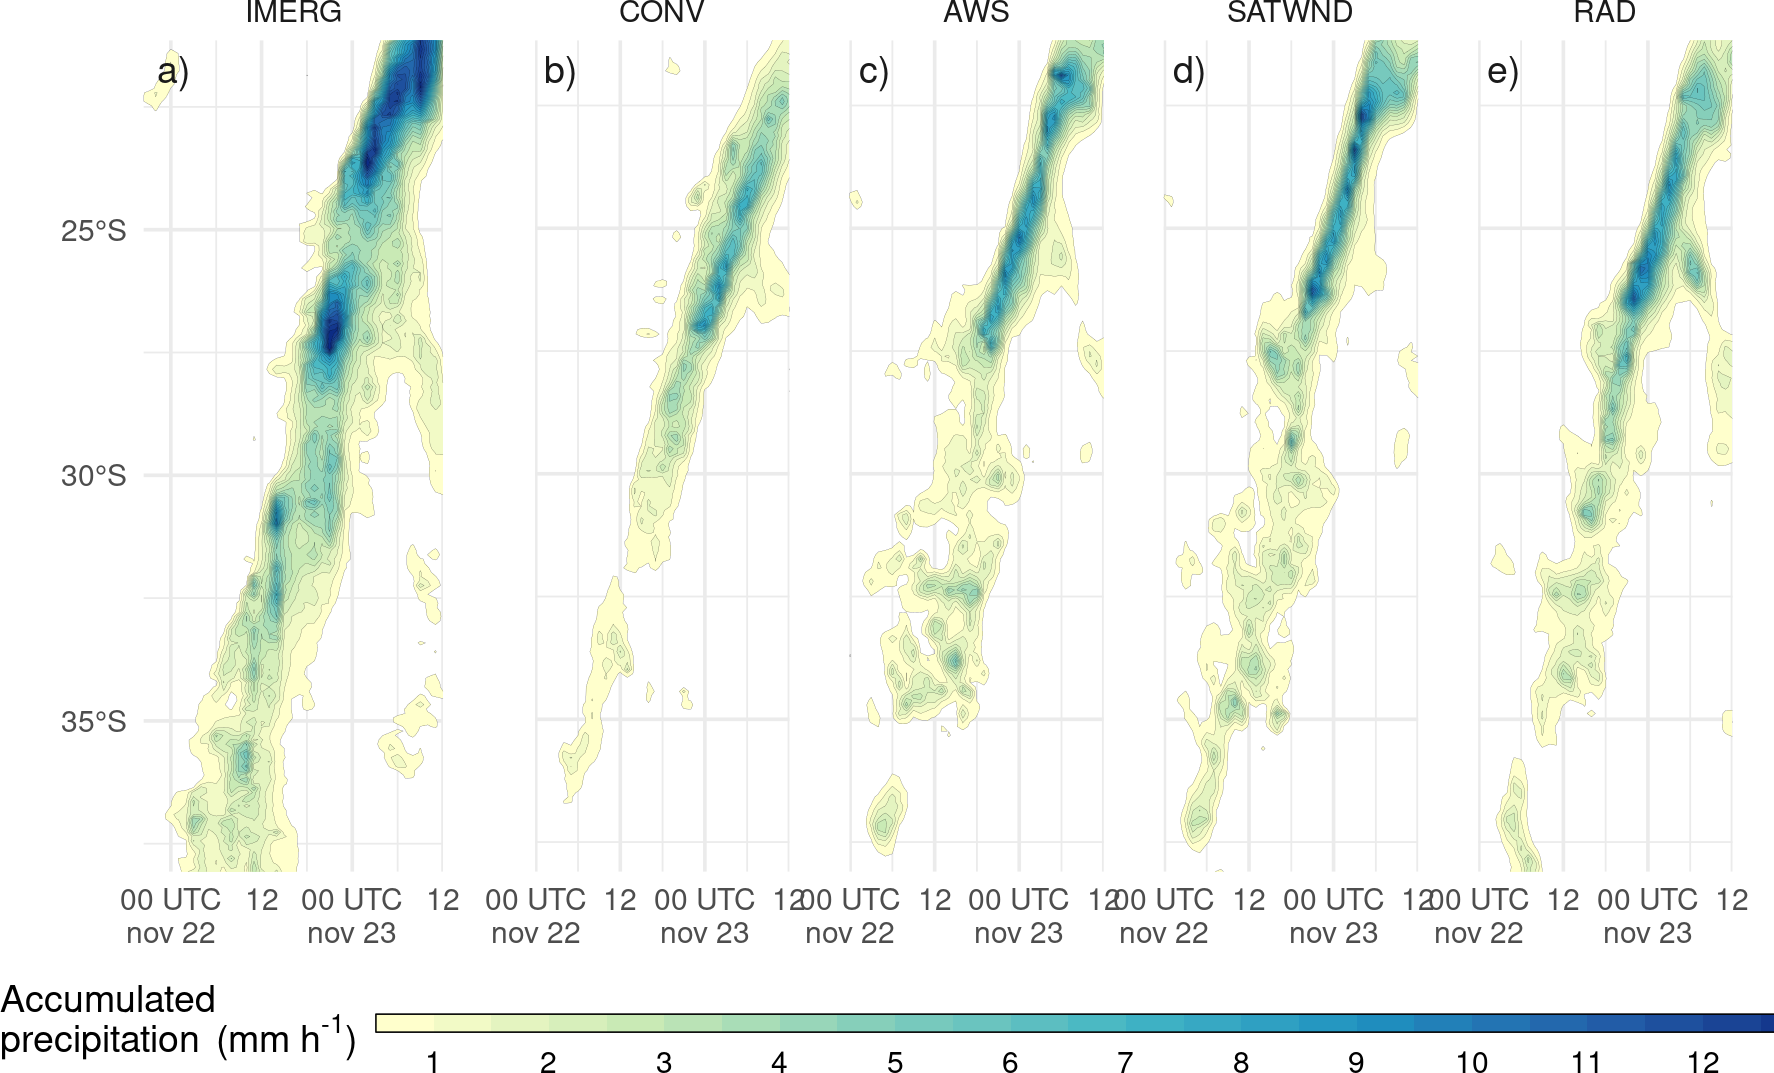
\includegraphics{../figures/pp-hov-1} 

}

\caption{Hövmoller diagram of probability matched mean hourly accumulated 1-h forecast precipitation for each latitude band estimated by IMERG (left) and simulated (right), for the ensemble mean of each experiment, averaged over a longitude range between 67\(^{\circ}\)W and 54.5\(^{\circ}\)W. Contours drawn every 0.5 \(mm\ h^{-1}\), starting at 0.5 \(mm\ h^{-1}\).}\label{fig:pp-hov}
\end{figure*}

The FSS is computed to quantify the spatial match between the observed precipitation and the first-guess hourly accumulated precipitation for the different experiments (Figure \ref{fig:fss}). For each threshold and spatial scale, Equation @red(eq:eq7) is applied in 6-hours rolling windows throughout the experiment period. All experiments show similar values of FSS during the initiation of the convection before 06 UTC Nov 22 except for RAD which performs better than the rest of the experiments during this period. This indicates that radiance observations have a positive impact on the analysis. The FSS for CONV is the lowest compared to the rest of the experiments and the differences are larger during the mature stage of the MCS. AWS and SATWND show similar FSSs indicating that satellite-derived wind assimilation has little impact on the precipitation for this case study. The assimilation of radiances led to an overall improvement of the 1-hour forecast precipitation, particularly for the 25 mm threshold during the period of heaviest precipitation on Nov 22 (Figure \ref{fig:fss}b,d). The enhancement is also important at the developing stage of the MCS (between 00 and 12 UTC Nov, 22 and also for spatial scales above 500 km, not shown).



\begin{figure}
\centering
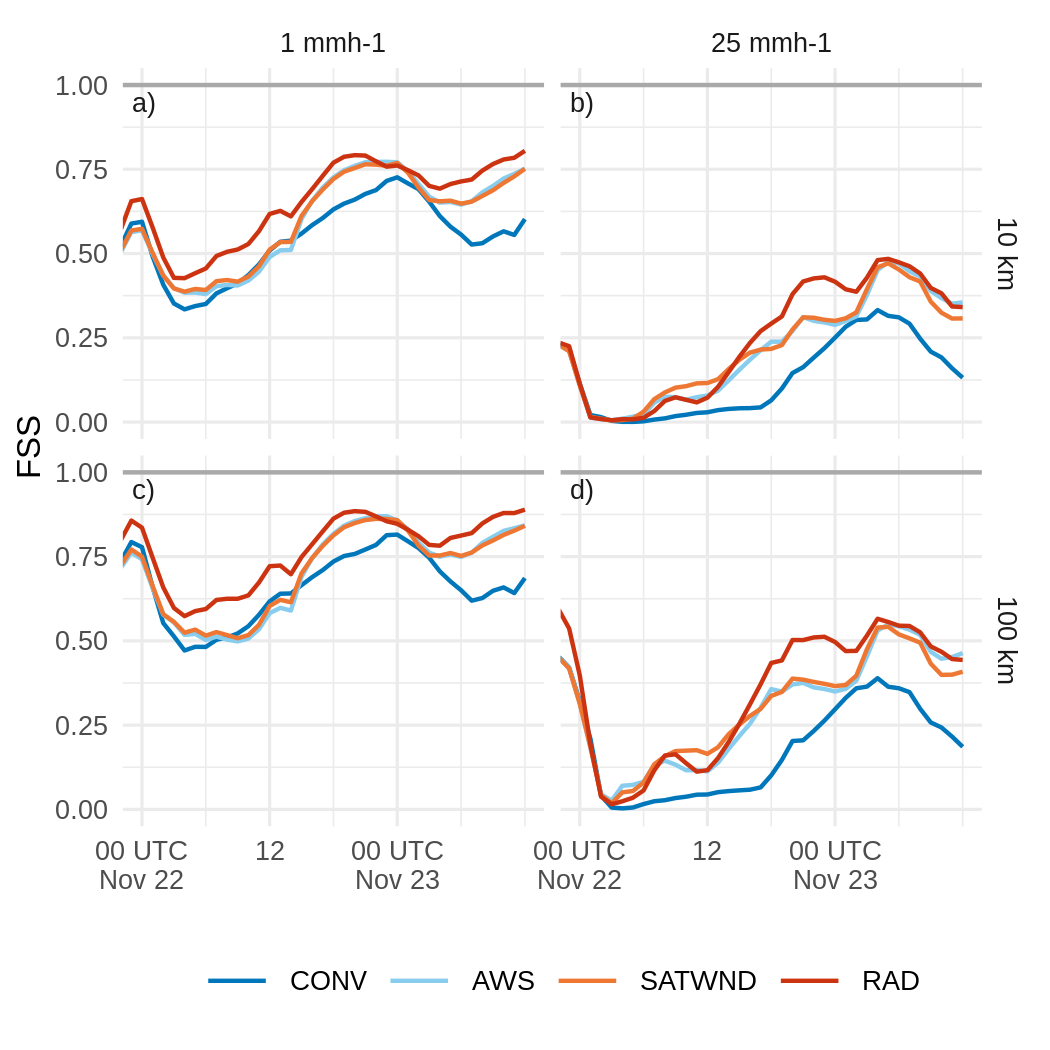
\includegraphics{../figures/fss-1.png}
\caption{\label{fig:fss}FSS calculated over 1-h forecast precipitation accumulated in a 6-hour moving window for 1 mm (a and c) and 25 mm (b and d) thresholds, on 10 km (a and b) and 100 km (c and d) scales, for the first-guess of CONV (blue line), AWS (light blue line), SATWND (orange line) and RAD (red line) experiments.}
\end{figure}

To complement the analysis, Figure \ref{fig:dbz-mean} shows the observed maximum reflectivity in the vertical column (COLMAX) and the ensemble mean COLMAX for the CONV and RAD experiments at different times between 10 and 19 UTC Nov 22. These experiments were chosen because they represent the analysis with the minimum (CONV) and maximum (RAD) number of assimilated observations. In addition, they are the worst (CONV) and best (RAD) performing experiments in terms of the 1-hour precipitation forecast skill (Figure \ref{fig:fss}). Overall, none of the short-range forecasts capture the mesoscale details in the reflectivity distribution. This is partially expected considering the coarse horizontal grid spacing (10 km), which is not enough to appropriately represent the strength of the convective band associated with the MCS. RAD better represents the observed features of the system showing a stronger and more organized MCS than CONV, over the domain center at 10 and 13 UTC (first and second columns in Figure \ref{fig:dbz-mean}). The convective cells that initiate after 16 UTC along the warm front in the northeast part of the domain are well captured by both experiments but are better represented in terms of strength in RAD. In addition, CONV captures the location of the MCS, but the convection seems to be less organized and much weaker than in RAD. Before and after the times shown in Figure \ref{fig:dbz-mean}, the agreement between location of the observed convective cells and the simulated in the experiment is quite good in the regions where radar data are available, especially for RAD.

Finally, Figure \ref{fig:soundings} shows the RMSE and bias calculated by comparing the experiments with radiosonde data from the RELAMPAGO missions, IOP 7 from 15 to 21 UTC Nov 21 (including 30 radiosondes), and IOP 8 from 14 to 20 UTC Nov 22 (including 22 radiosondes).

IOP 7 (Figures \ref{fig:soundings}a-d) provides a good characterization of the pre-convective environment during the first day of our experiments. The area where the observations were taken was characterized by mostly clear skies and a low-level northerly flow associated with warm and moist advection. In general, the experiments show a similar RMSE and bias for all the variables. AWS observations were able to reduce the RMSE for temperature and dew point temperature in the PBL and reduce a small dry bias. However, in this region (Figure \ref{fig:dominio}b) and for this period, AWS increments (Figure \ref{fig:UV-diff}d) degrades the zonal wind between 7 and 12 km increasing the bias and RMSE (Figure \ref{fig:soundings}c).



\begin{figure*}[ht]
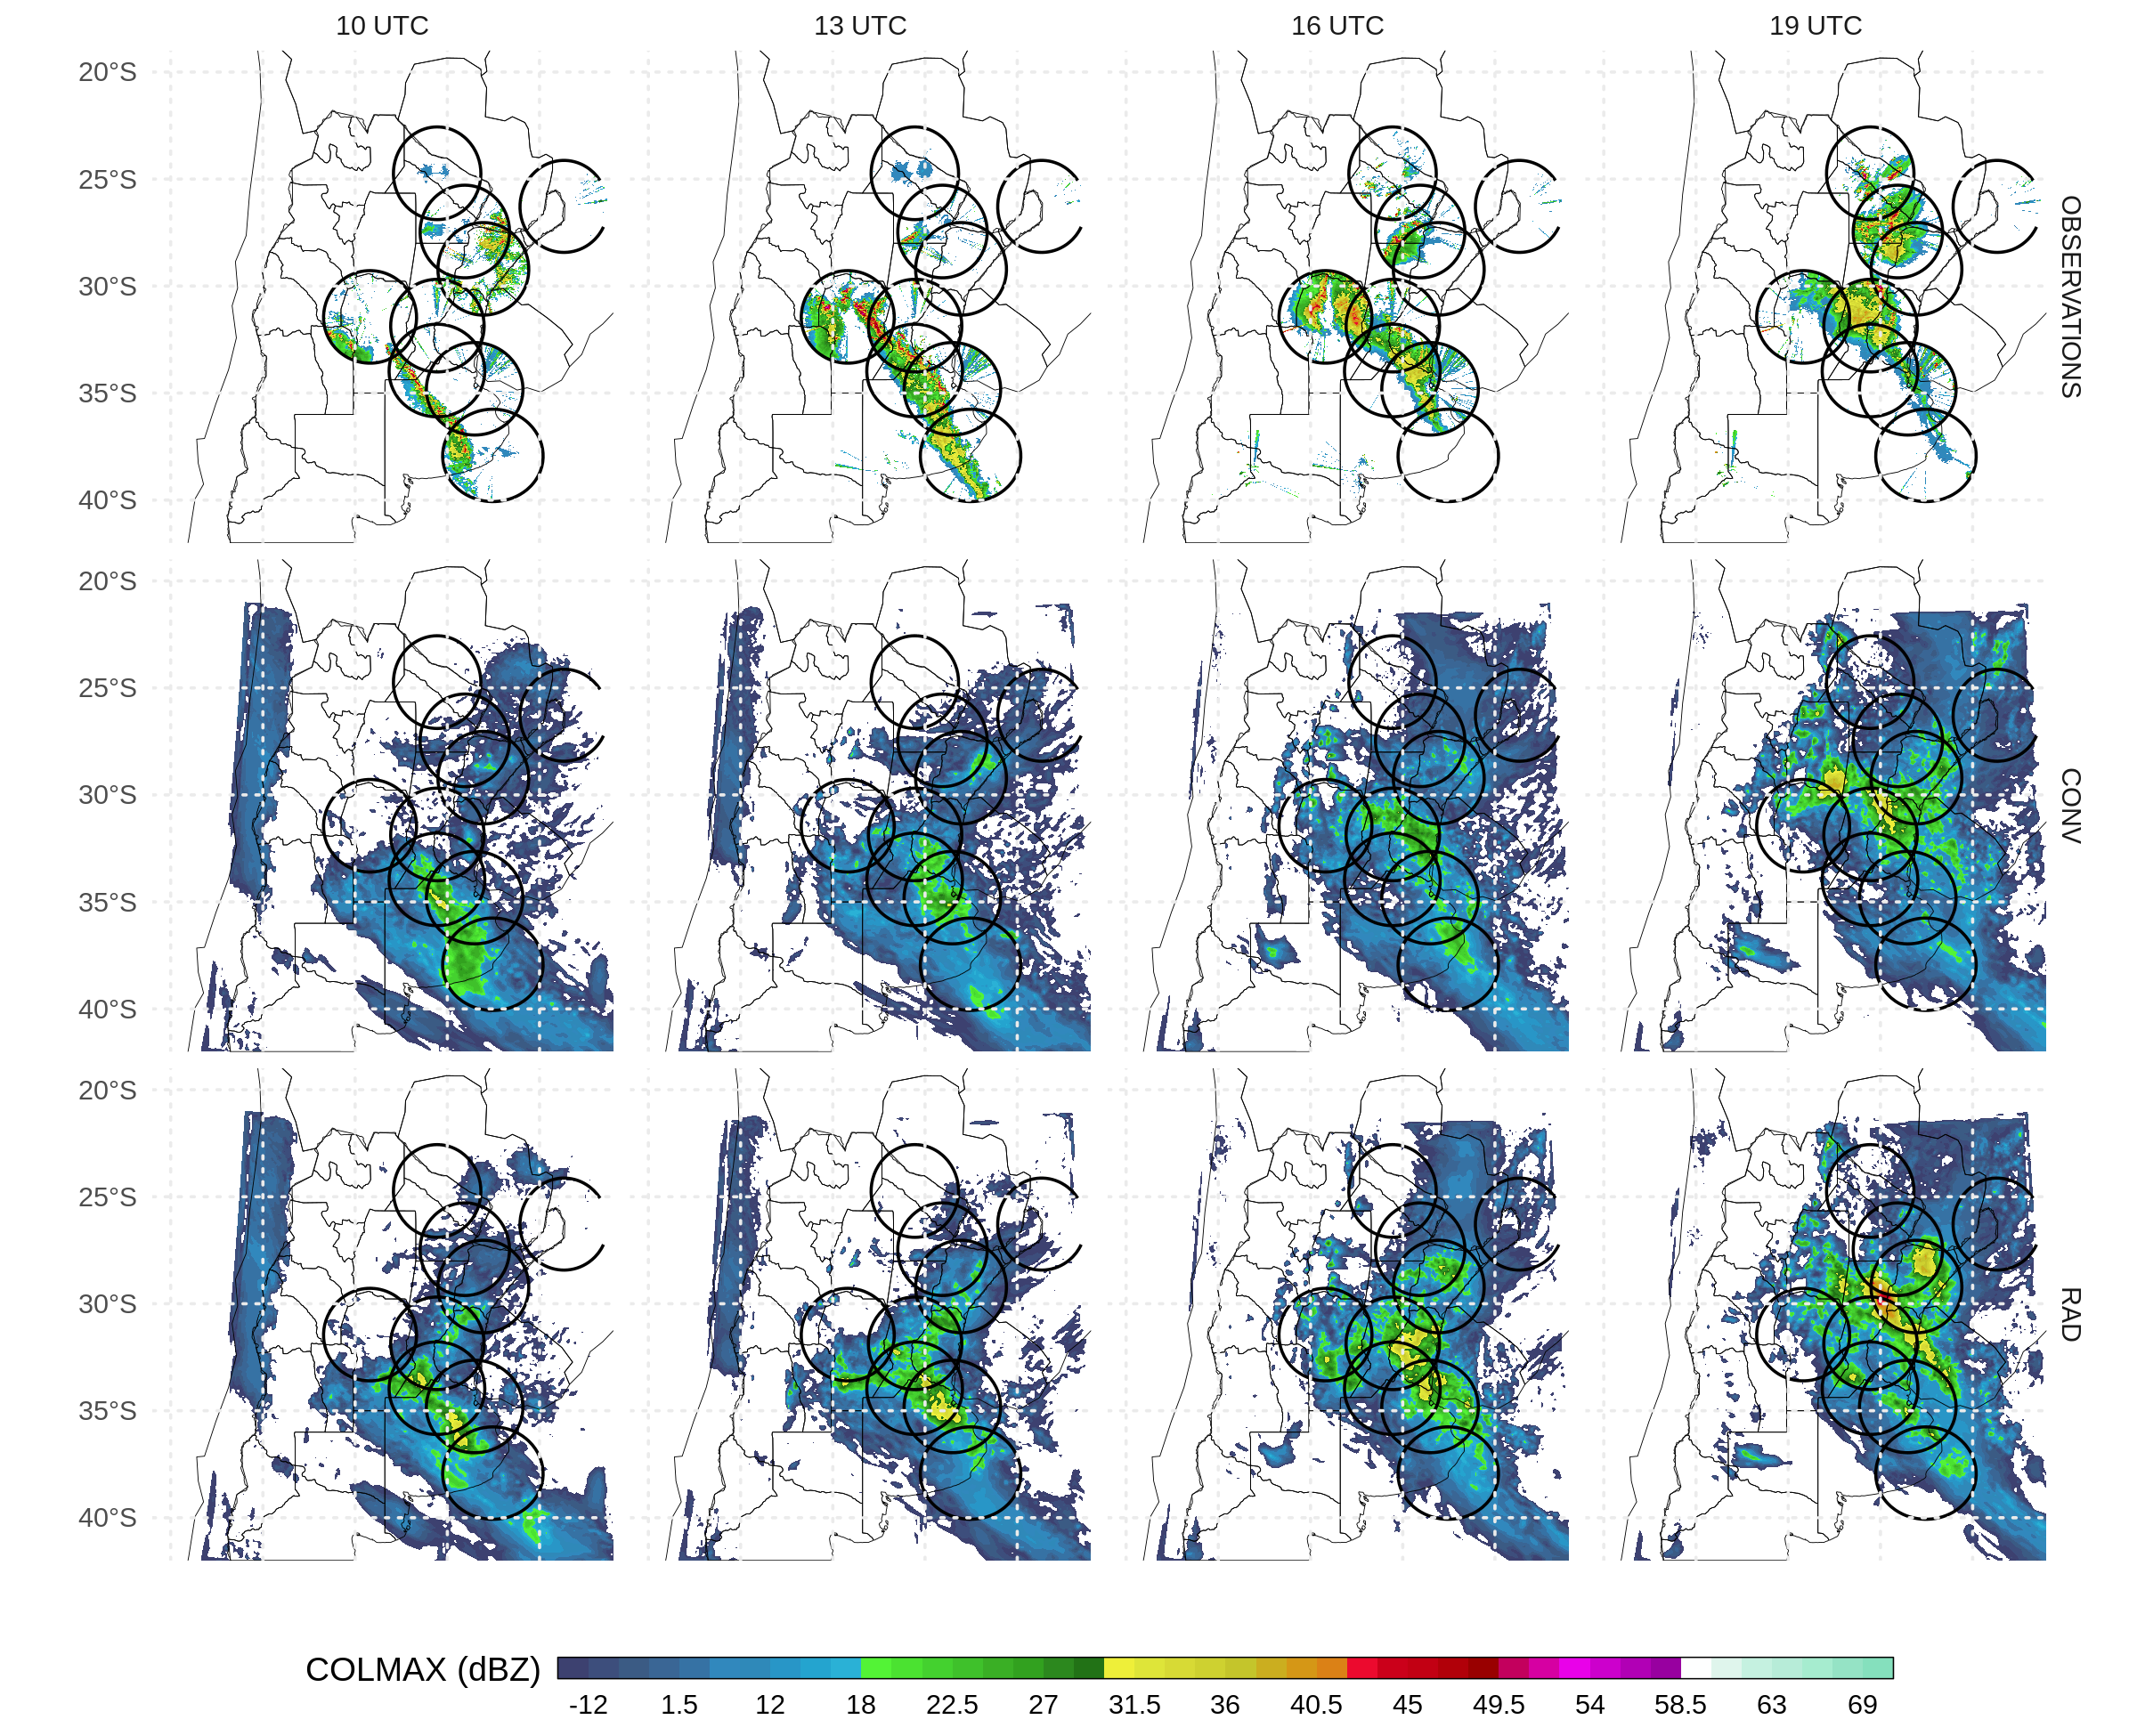
\includegraphics[width=1\linewidth]{../figures/dbz-mean-1} \caption{Maximum reflectivity in the column (COLMAX in \(dBZ\)), observed (upper row) and 1-hr forecast probability matched mean column maximum reflectivity for CONV (second row) and RAD (third row) at 10 UTC (first column), 13 UTC (second column), 16 UTC (third column), and 19 UTC (fourth column) Nov 22, 2018. Black circles in first row show the observation range of each radar.}\label{fig:dbz-mean}
\end{figure*}

For IOP 8 (Figures \ref{fig:soundings}e-h), the densely observed area was behind the MCS, but far enough from it to not be directly affected by its mesoscale circulation. This area was also behind the cold front and affected by low-level cold advection. The assimilation of AWS, SATWND, and RAD reduces the cold bias and RMSE for temperature between 5 and 12 km and the RMSE in the PBL compared with CONV (Figure \ref{fig:soundings}e). The reduction of bias and RMSE is also important for dew point temperature (Figure \ref{fig:soundings}f) with SATWND showing the biggest impact followed by AWS and RAD. The zonal wind is overestimated in the analyses and only RAD shows an improvement with respect to CONV in the upper troposphere (Figure \ref{fig:soundings}g). At low levels the meridional wind (Figure \ref{fig:soundings}g) presents a negative bias, indicating an underestimation of the southerly wind behind the cold front principally in AWS, SATWND, and RAD. In fact, low level biases in these experiments are higher than in the CONV experiment, indicating a detrimental effect of the additional observations (possibly associated with the effect of AWS).



\begin{figure*}[ht]

{\centering 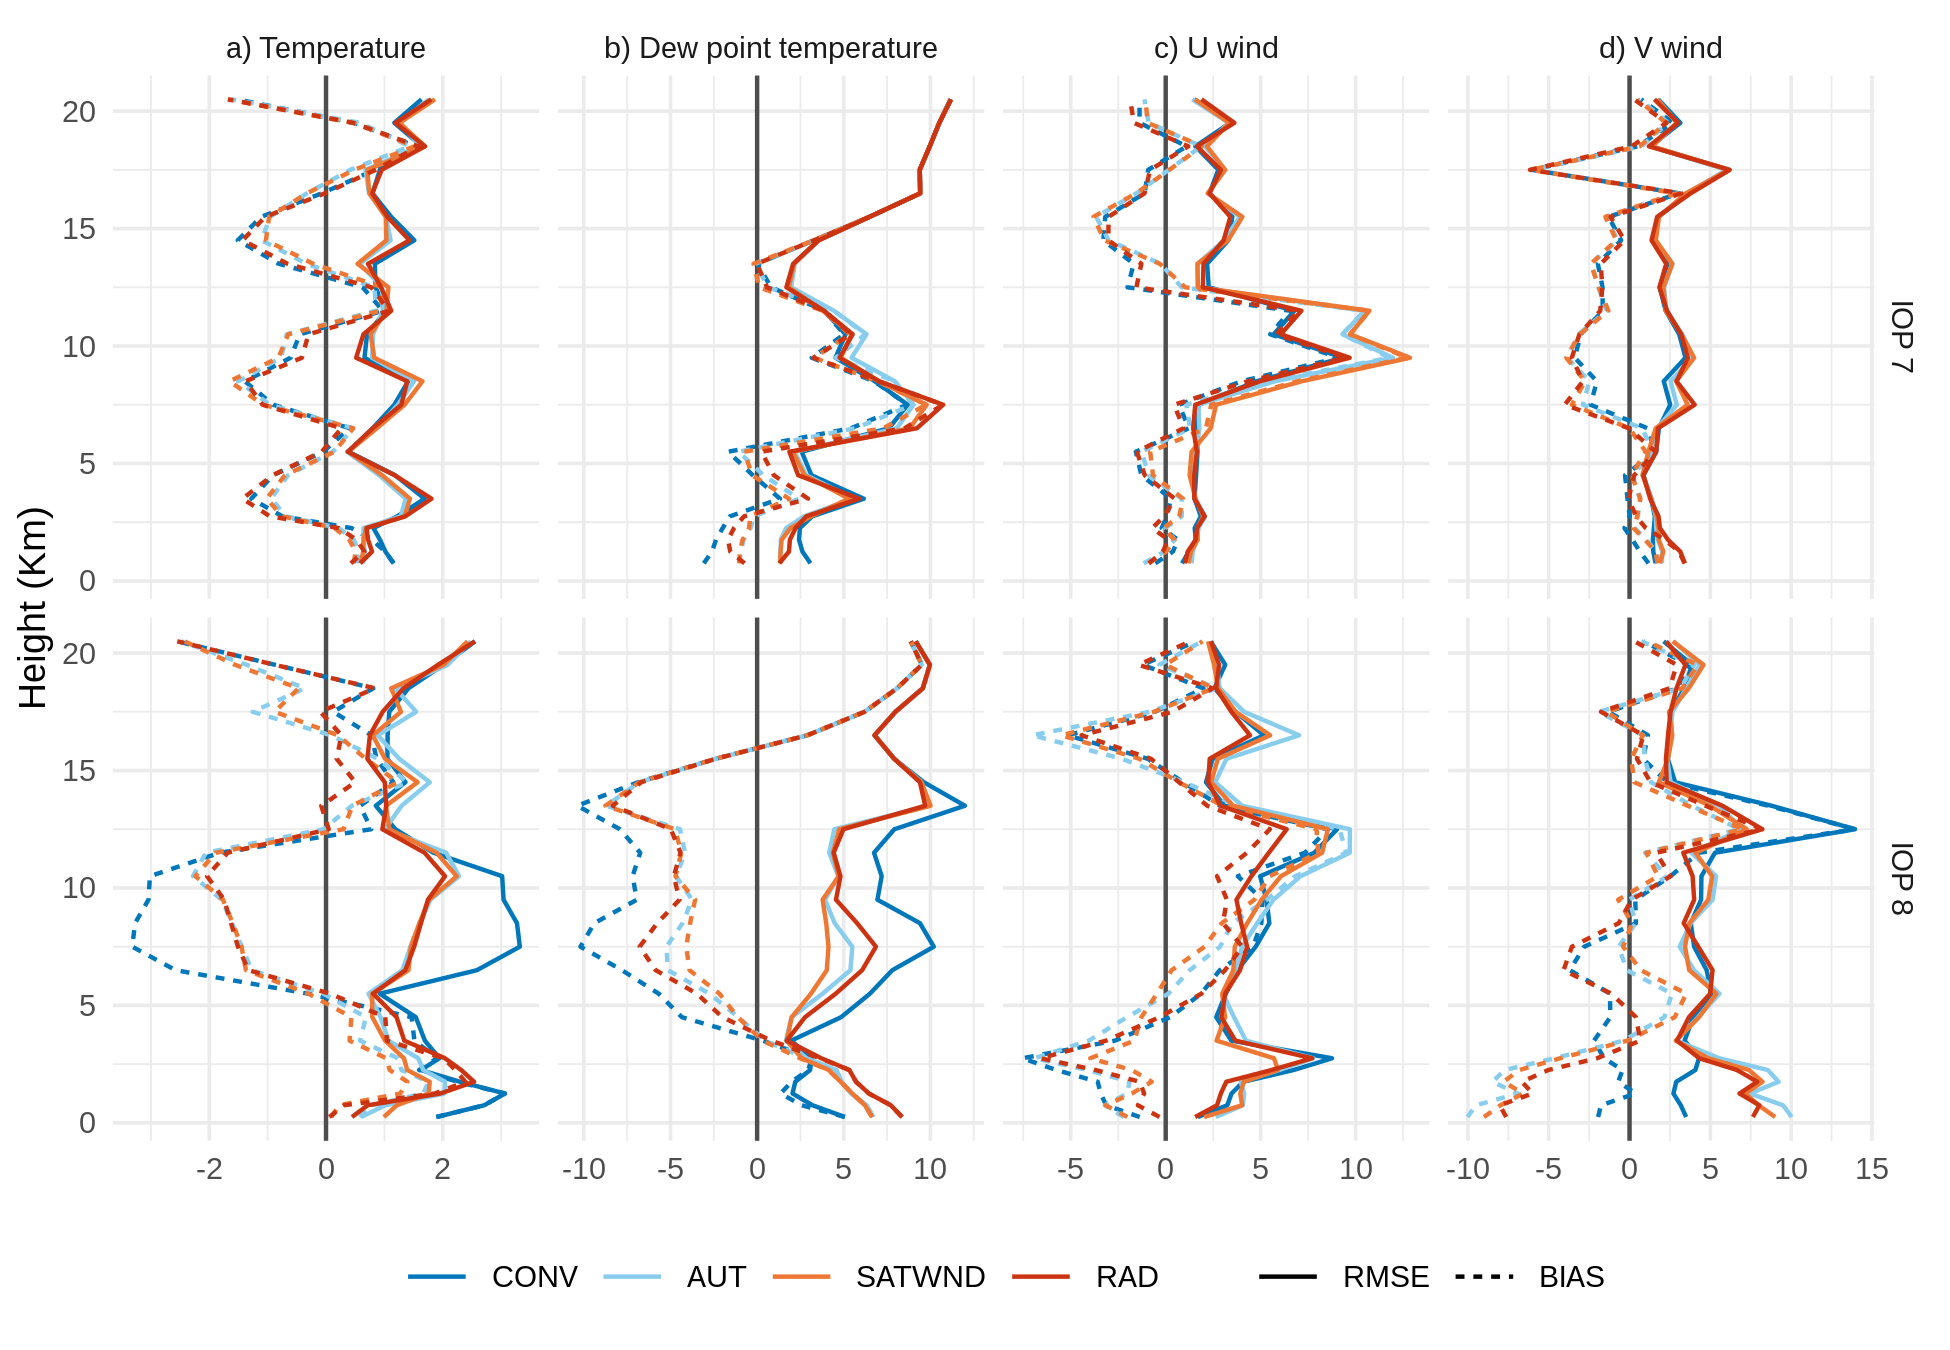
\includegraphics{../figures/soundings-1} 

}

\caption{RMSE (solid line) and Bias (dashed line) of a) temperature (\(K\)), b) dew point temperature (\(K\)), c) u wind (\(m\ s^{-1}\)) and d) v wind (\(m\ s^{-1}\)) calculated by comparing the analysis of each experiment with the RELAMPAGO soundings during IOP 7 and IOP 8. The blue line corresponds to CONV, the light blue line to AWS, SATWND is represented with an orange line, and RAD with a red line.}\label{fig:soundings}
\end{figure*}

\hypertarget{ensemble-forescast-validation}{%
\subsection{Ensemble forescast validation}\label{ensemble-forescast-validation}}

This section analyzes the 60-member ensemble forecast initialized at 00 and 06 UTC Nov 22 from each experiment that runs for 36 and 30 h respectively, until 12 UTC Nov 23. The FSS is again calculated for the ensemble forecasts in 6-hour rolling windows for the same thresholds and spatial scales as for the first-guess hourly accumulated precipitation to quantify the skill of the forecasts to predict precipitation (Figure \ref{fig:fssfcst}). CONV forecasts perform very poorly in terms of the FSS compared with the experiments that include other sources of observations. AWS, SATWND, and RAD show improvements in the FSS values, particularly for the higher threshold (Figure \ref{fig:fssfcst}b, d). Moreover, the late initialization at 06 UTC performs better for AWS, SATWND, and RAD than the forecast initialized at 00 UTC, highlighting the positive impact of the observations assimilated between 00 and 06 UTC.

The satellite-derived wind observations show a clearly positive impact on the forecast, in contrast to what was seen when comparing the 1-h forecast with independent observations in terms of precipitation. Conversely, the radiance observations resulted in a neutral to a slightly negative impact on the forecast as opposed to what was seen when comparing the 1-h forecast to IMERG estimations. The reason why the forecasts initialized from RAD degrade over time needs to be further study. However, it is possible that the assimilation of observations associated with channels affected by the surface is contributing to the degradation of the PBL in the analysis and subsequently in the forecasts. \citet{lim2014} observed limited impact when assimilating AIRS observations and attribute this result to the use of surface channels where the uncertainties associated with emissivity are large.



\begin{figure}
\centering
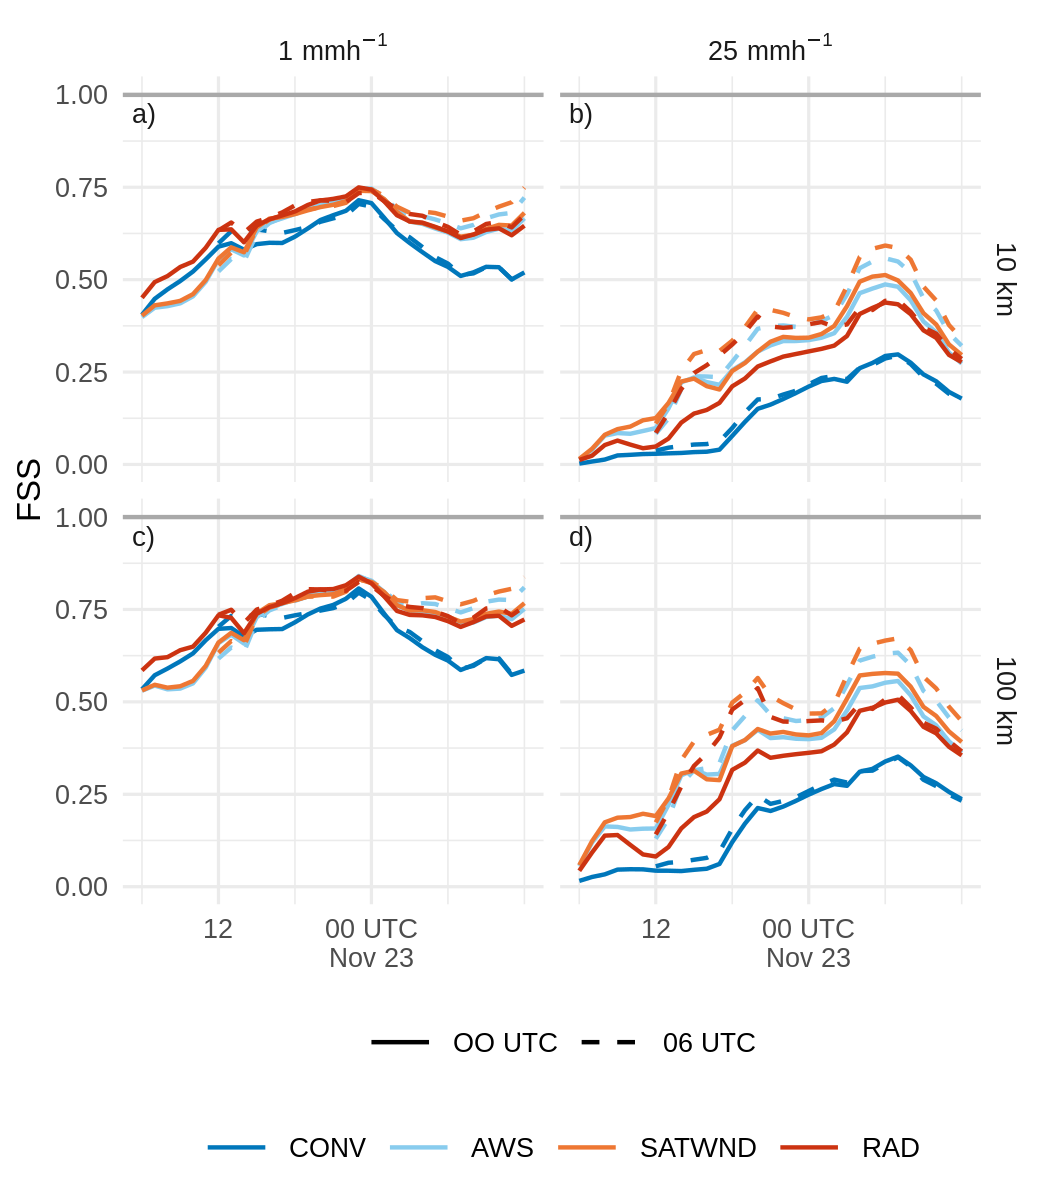
\includegraphics{../figures/fssfcst-1.png}
\caption{\label{fig:fssfcst}FSS calculated over a 6-hour moving window for 1 mm (a and c) and 25 mm (b and d) thresholds, on 10 km (a and b) and 100 km (c and d) scales, for the forecasts initialized from CONV (blue line), AWS (light blue line), SATWND (orange line), and RAD (red line) experiments at 00 UTC (solid line) and 06 UTC (dashed line), Nov 22.}
\end{figure}

\hypertarget{conclusions}{%
\section{Conclusions}\label{conclusions}}

Southern South America is a particularly interesting region due to the heterogeneity in topography and coarse resolution of the operational observing network (considering both surface based and upper air observations). This, combined with a climatology characterized by frequent organized convective events makes mesoscale DA particularly challenging. This paper investigates, for the first time in South America, using a case-study approach, the impact of different observation systems on the performance of an ensemble-based mesoscale regional DA system. This case study corresponds to a massive MCS that developed over Southern South America on Nov 22, 2018 during the RELAMPAGO field campaign. In particular, the impact on the analysis quality of assimilating frequent and relatively dense surface observations, satellite-derived winds, and satellite clear-sky radiances from multiple sensors is explored.

Firstly, the consistency of the ensemble was evaluated to ensure a good agreement between the ensemble spread and the observational errors with respect to the distance between the ensemble mean and the observations. While conventional observations departures are consistent with the ensemble spread and assumed observation errors, satellite-derived winds and radiance observations departures are lower than expected. The latter could be the result of an overestimation of the observation errors which is usually introduced to avoid the detrimental impact on the analysis of poor quality observations.
In this case study, all the observation types considered (i.e.~automatic weather stations, satellite derived winds and clear-sky radiances from polar orbiting satellites) improves the quality of the analysis and of the short range forecast with respect to the conventional observation network. In terms of the analysis, automatic weather station observations, which have high spatial and temporal resolution, produced impacts mainly within the PBL but which occasionally extends throughout the troposphere during the periods where moist convection is stronger within the domain. These observations also helped to reduce the warm and dry bias present in the model, producing an analysis closer to the ERA5 reanalysis. During the pre-convective environment, assimilating surface temperature, dew point temperature, and meridional wind improved the analysis at low levels when compared with observed soundings. In particular, when these observations are assimilated, precipitable water content and low level meridional circulation led to the enhancement of deep convection and heavy precipitation which is closer to observations.

Positive results were also found when assimilating radiance observations, which produced a better development of the convection and its associated outflow circulation, mainly during the mature stage of the MCS, leading to increased accumulated precipitation compared to the case in which these observations are not assimilated. However, these observations weakened the impact of automatic weather station observations within the PBL, slightly increasing the warm and dry bias with respect to ERA5. While this needs to be further studied, it could be related to the assimilation of channels affected by the surface or sub-optimal bias correction. Comparing the experiment with independet soundings, the assimilation of radiances improved mid and upper level wind.

The assimilation of satellite-derived wind did not produce a noticeable impact on the analysis. This is possibly due to the relatively small number of observations in low levels available for this case study and their large observation error. However, there are improvements in the 1-h forecast accumulated precipitation distribution. A more comprehensive analysis is necessary to understand the mechanisms behind the impact of these observations on longer range forecasts.

The evaluation of the performance of independent ensemble precipitation forecasts initialized from the analyses during Nov 22 showed that the forecasts initialized from AWS, SATWND, and RAD were able to forecast the precipitation substantially better than CONV. In particular, continuous assimilation of satellite-derived wind and radiance observations improved the latest initialization but only satellite-derived wind observations produced a positive impact that persisted throughout the forecast. Why the forecast initialized from RAD did not perform better than SATWND needs to be further study.

To summarize, in this case study we found that the assimilation of surface observations with high spatial and temporal resolution, satellite-derived winds, and clear-sky radiances from polar orbiting satellites had an overall positive impact on the development of the studied MCS and its associated precipitation. Moreover, ensemble forecasts initialized from the analysis showed promising results for predicting extreme severe precipitation events. In the future, we will further analyze the impact of these observations upon short-range forecasts over longer periods and evaluate the assimilation of other sources of observations such as GPS radio occultation data and radiances from geostationary orbiting satellites like GOES-16.

\hypertarget{code-and-data-availability}{%
\section{Code and data availability}\label{code-and-data-availability}}

A version-controlled repository of the code used to create this analysis, including the code used to download the data can be found at \url{https://github.com/paocorrales/mesoda}. The derived data that support the findings of this study are also openly available in Zenodo at http://doi.org/10.5281/zenodo.7015913, version 0.9.2.

\hypertarget{acknowledgments}{%
\section*{Acknowledgments}\label{acknowledgments}}
\addcontentsline{toc}{section}{Acknowledgments}

We are very thankful to the Atmospheric and Sea Research Center (CIMA), the University of Buenos Aires (UBA), and the National Scientific and Technical Research Council (CONICET) who support this study. We acknowledge the Sistema Nacional de Radares Meteorológicos supported by the Secretaría de Infraestructura y Política Hídrica for kindly providing the radar observations used for validation and the National Meteorological Service for facilitating the access to the data. We also acknowledge the Cheyenne HPC resources (doi:10.5065/D6RX99HX) from NCAR's Computational and Information Systems Laboratory, National Science Foundation (project code UIUC0012). Also, PICT 2017-2233 and PICT 2018-3202 projects of the National Agency for the Promotion of Research, Technological Development and Innovation from Argentina partially funded this project.

\renewcommand\refname{References}
\bibliography{paperANA.bib,packages.bib,era.bib}


\end{document}
